\documentclass[british,titlepage,oneside]{project_setup}

\addbibresource{bibliography.bib}


% From https://www.overleaf.com/learn/latex/Glossaries

\makeglossaries % Prepare for adding glossary entries


\newglossaryentry{latex}
{
        name=latex,
        description={Is a mark up language specially suited for
scientific documents}
}

\newglossaryentry{bibliography}
{
        name=bibliography,
        plural=bibliographies,
        description={A list of the books referred to in a scholarly work,
typically printed as an appendix}
}

\newglossaryentry{maths}
{
    name=mathematics,
    description={Mathematics is what mathematicians do}
}


% --------------------
% ----- Acronyms -----
% --------------------

\newacronym{phd}{PhD}{philosophiae doctor}
\newacronym{CoPCSE}{CoPCSE@NTNU}{Community of Practice in Computer ScienceEducation at NTNU}
\newacronym{gcd}{GCD}{Greatest Common Divisor}

\newacronym{ai}{AI}{Artificial Intelligence}


 % add glossary and acronym lists before document

\begin{document}
\setstretch{1.2}

\chapter*{Abstract}

A condensation of the essential information of the article.
\chapter*{Sammendrag}

Sammendraget skal være \textit{Abstract} på norsk.

\chapter*{Preface}

Builds on Project thesis \cite{project_thesis}.

Some chapters are marked with *

Expects that ML is known and is written from a ML and cybernetics perspective. 

New project -- first in PyTorch 
\chapter*{Acknowledgements}

Thank you for help and guidance
- learning stuff, tips to learn pytorch, dataset, discussion of VAE, ppo results
- environment and PPO results


Thanks for patience

Thanks for a cool master

Thank you for PC

Thanks to the boys for moral support, Gina and family

\tableofcontents
\listoffigures
\listoftables
%\lstlistoflistings

\printglossary[type=\acronymtype] % Print acronyms
\printglossary                    % Print glossary

\chapter{Introduction}
\label{chap:1_introduction}

\section{Motivation}
Autonomous navigation of robotic vehicles is a complicated task that has challenged the cybernetics community since its inception.
It is a research field of substantial focus particularly in recent years, given its novel applications within commercial sectors \cite{eelumeSale, anymalInTheField, CogniteVisualInspection}, transportation \cite{autoferryNTNU}, search and rescue \cite{washingtonPost}, and defence \cite{darpaAutonomy}. As new possibilities for autonomy are increasing, so is the need to find new, innovative, robust and safe solutions to meet this demand.

The difficulty of autonomous navigation in cluttered and dynamic environments arises from the combination of three separate tasks: first to perceive the local environment directly from on-board sensors, then to predict how the environment will evolve, and finally to decide on a safe and intelligent action based on the inferred information \cite{darpaCar}. Each of these tasks presents its challenges, such as dealing with noise or uncertainty in sensor data or feasible trajectory planning, but separating these tasks into a threefold process ultimately leads to an increased latency and compounding of errors in the pipeline \cite{HighSpeedFlightWild}.

Moreover, as robotic use-cases are becoming more advanced -- such as in underwater \cite{eelume}, forested \cite{HighSpeedFlightWild} and subterranean environments \cite{GBplanner} -- autonomous robots now have to contend with environments that are: sensor-degraded with limited illumination; long, narrow and multi-branching; unpredictable and unstructured; isolated from external communications. Though localisation and mapping techniques based on 3D perception have been successful in unstructured environments in the past \cite{navigationSLAM}, the characteristics of these newer domains present new challenges for traditional approaches. Specifically, these environments make it difficult to maintain an accurate map of the environment, puts the tractability of trajectory planning into question and limits the amount of computational resources available to the robot \cite{LearningStateRepresentation, NavRep_unsupervised, HighSpeedFlightWild, LBplanner}.

Not to mention, navigation within cluttered environments requires fast, accurate and careful planning of versatile vehicles -- such as in multirotor aerial vehicles (quadrotors) \cite{MultirotorAerialVehicles}. This requires a quick mapping from sensor data to action, which makes a high-latency solution non-viable because of the inherent difficulty of pose estimation when travelling at high speeds \cite{NavRep_unsupervised, HighSpeedFlightWild}. 

Therefore, these issues prompt the consideration of learning-based methods to directly infer actions from raw sensor input, as an alternative to the three-subtask, model-based pipeline. The idea is to remove the necessity for accurate maps, though retaining essential features, and using this to plan feasible trajectories even in complex edge-case scenarios.
Utilising a data-driven approach should allow an agent to capture the system's dynamics and the environment's uncertainties without the need for any explicit programming \cite{RLinRoboticsSurvey} -- thus removing the need for feature engineering or heuristics to make the navigation task tractable \cite{LearningStateRepresentation}. 
The processing time dramatically decreases due to this direct mapping, as sensor data does not need to be preprocessed into higher dimensional information \cite{fan2018distributed, stereoCamTracking}, maps will not have to be generated or queried, and exhaustive collision checking is avoided \cite{LBplanner}.
Instead, a learning approach will be used to extract high-dimensional information directly, capable of filtering out redundant information in LiDAR and depth data. Then, the agent can learn collision avoidance based on experience from these high-level features \cite{LearningStateRepresentation}. 

The apparent limitation of using learning-based methods is that the amount of data required to solve complex tasks is proportional to its complexity \cite{LearningWalkMassivelyParallel}, where varied environments are often also required in the learning process \cite{RichEnvironments}. Due to this, the question of whether or not a task was learnable through reinforcement learning became simply a question of time or computational resources. If these resources were unavailable, more sample-efficient methods had to be explored, for example: supervised learning through clever use of datasets \cite{cad2rl, dronet}, engineering of action spaces and learning these in a self-supervised manner \cite{deepCollisionPredictorOracle}, or by imitation learning using an expert planner \cite{LBplanner, pfeiffer2017perception, HighSpeedFlightWild}.

However, until recently, the research community has been developing parallel end-to-end hardware-accelerated (GPU) simulators, such as \textit{Isaac Gym}, which have provided the opportunity to simulate tens of thousands of environments in parallel and ``enables the solving of tasks with a single GPU that were previously only possible on massive CPU clusters'' \cite{IsaacGym}. This has opened up a multitude of possibilities for autonomous navigation using reinforcement learning, thus being the motivation for this thesis.


\section{Scope}
This thesis explores how a mapless navigation policy for collision avoidance can be learned on a quadrotor without expert demonstrations by leveraging novel ideas in learning-based autonomous navigation combined with a massively parallel learning scheme (Isaac Gym). 
Specifically, the aim is to infer a reference velocity and steering angle for the quadrotor given its state and depth image from a forward-facing depth camera. With this policy, an agent should be able to navigate through a cluttered environment to a goal specified in three-dimensional space.

To learn this policy, this thesis will present the theory and implementation of a two-part deep neural network module. The first module, a variational autoencoder (VAE), is tasked with extracting the essential information from a depth image. The second module will be a fully-connected neural network (or multi-layer perceptron) and serves as the reinforcement learning agent. The agent will receive the essential information of the depth image (i.e. its features), along with the quadrotor state, and decide on a velocity and yaw rate reference for the quadrotor. To optimise the agent, the Proximal Policy Optimisation (PPO) algorithm will be used. 

Additionally, as the VAE and simulation environment is set up from scratch, the design choices for each module will also be discussed in light of intermediate results during the development phase.
For the VAE, this includes the choice of architecture and loss functions for improvements in the reconstructed images.
For the MLP, this includes simulation setup and gradual training steps (curriculum) to achieve a stable training process and eventually collision avoidance.

Finally, the intermediate and final agents will be tested in cluttered environments with varying difficulty, where their success (and failure) will be analysed. 

\todo{example of results,
video and link}


\section{Outline}

The outline of this thesis will be as follows:
\vspace{2mm}
\begin{itemize}
    \item \textbf{Chapter 1: Introduction} \\
    Motivation for this thesis is presented, along with the ... \vspace{3mm}

    \item \textbf{Chapter 2: Theoretical Background}
    \vspace{3mm}
    
    \item \textbf{Chapter 3: Related Works} 
    \vspace{3mm}
    
    \item \textbf{Chapter 4: Problem Formulation} 
    \vspace{3mm}
    
    \item \textbf{Chapter 5: Proposed Approach}
    \vspace{3mm}
    
    \item \textbf{Chapter 6: Implementation} 
    \vspace{3mm}
    
    \item \textbf{Chapter 7: Navigation Policy Evaluation Studies} 
    \vspace{3mm}
    
    \item \textbf{Chapter 8: VAE Evaluation Studies} 
    \vspace{3mm}
    
    % \item \textbf{Chapter 9: Discussion} 
    \vspace{3mm}
    
    \item \textbf{Chapter 9: Conclusions} \vspace{3mm}
    
\end{itemize}






\chapter{Theoretical Background}
\label{chap:2_background}

% VAE
% PPO
% 15pages


\section{Variational Autoencoder}

\subsection{Autoencoder}

\subsection{Convolutional Variational Autoencoder}


\section{Reinforcement Learning}

\subsection{Proximal Policy Optimisation}
\chapter{Related Works}
\label{chap:3_related_works}
\begin{comment}
There is extensive prior work in learning-based methods for autonomous navigation. Together, they encompass a variety of methods, from model-based to model-free, applied in environments including land, air, cluttered and dynamic. 
Despite these differences, the challenge of learning-based autonomous navigation is usually approached through the same three questions:
\begin{enumerate}
    \item How can the environment be perceived? 
    \item What actions can be taken? 
    \item How can these be learned?
\end{enumerate}
\end{comment}

In the complex task of autonomous navigation, learning what to do or which actions to take -- such as the optimal velocity and steering angle for a given input image -- can be challenging to express explicitly. In this chapter, we will explore some related learning-based methods to tackle this problem, covering methods that utilise expert demonstrations in supervised or imitation
learning, or those that rely on a reinforcement learning approach to learn an optimal behaviour.

\section{Motion Planning with Supervised Learning}
\label{sec:3_supervised_learning}
The first learning-based method for navigation is to supervise the learning process by compiling a set of expert demonstrations. The idea here is that we have some deep NN -- typically a CNN -- that will learn to directly predict optimal actions (or action sequences) based on some input -- typically an image from an RGB or depth camera or laser range findings from a LiDAR sensor. In this approach, the navigation problem is essentially a prediction problem. The main challenge is defining the optimal target action for each input when compiling the dataset of expert demonstrations.

In \cite{pfeiffer2017perception}, they proposed the first target-oriented end-to-end navigation model for a robotic platform, capable of predicting steering commands -- translational and rotational velocities -- from raw 2D-laser range findings and a target position. They use a CNN with residual blocks inspired from \cite{KaimingResNet}, which takes in the LiDAR data and concatenates this feature output with the target position to serve as an input to a fully connected NN. Then, comparing the action prediction from this model to targets from a global planner -- serving as an expert -- allowed \cite{pfeiffer2017perception}  to train their model in an end-to-end fashion. By using a global planner, the authors also avoided requiring a human expert to tediously provide steering commands at a large scale.

In \cite{dronet}, they introduced \textit{DroNet} -- an efficient CNN with a ResNet8 architecture also from \cite{KaimingResNet} -- that can guide a quadrotor in urban environments by predicting steering angles and corresponding collision probabilities from single image inputs. To manage this, \cite{dronet} utilised a dataset created from cars and bicycles to train their CNN instead of compiling their own dataset.
From this, they achieved safe navigation that was highly generalisable and avoided the high sample complexity required for reinforcement learning algorithms.

In autonomous drone racing, one requires a fast perception system capable of real-time detection and pose estimation of gates. This problem can also be approached with a CNN, which then requires the design of a custom dataset due to highly varying race tracks and possible actions. In \cite{supervised_DeepDroneRacing}, they proposed a method of generating a labelled dataset using an expert trajectory and policy. First, an optimal trajectory can be generated through all gates if their poses are known.
With this trajectory, an expert policy can be used to generate a desired direction and speed to follow the trajectory. Finally, by collecting sampling state estimates and corresponding images, one could use the expert policy to label the images to create a labelled dataset. This allowed \cite{supervised_DeepDroneRacing} to train a CNN -- a DroNet from \cite{dronet} -- to learn the desired direction and speed output for each image input. 

\section{Motion Planning with Semi-Supervised Learning}
\label{sec:3_semi_supervised_learning}
Self-supervised learning techniques are closely related to supervised methods, requiring a labelled dataset so to be able to learn desirable actions for inputs. However, this approach does not depend on some expert planner's demonstrations. In contrast, these methods rely solely on a robot's retrospective self-experience to learn the environment's physical attributes.
For example, \cite{learning_to_fly_by_crashing} relies on learning a navigation policy through crashing. They equipped a 720p camera to a quadrotor and tasked it with flying in a straight line until collision. Based on the experience gathered from this simple behaviour, they compiled an image dataset full of positive and negative collision examples and used this to train a CNN to predict whether or not to go straight. By further cropping the images into left and right halves, they created a turning mechanism that allowed the quadrotor to navigate cluttered indoor environments.

The work done in \cite{Badgr} takes this concept further, teaching a mobile ground robot through self-supervision to navigate in ``real-world urban and off-road environments with geometrically distracting obstacles'' with only a camera. The Berkeley autonomous ground robot, \textit{BADGR}, gathers off-policy data in real-world environments from a random control policy and uses this to train a deep model -- a CNN and Long Short-Term Memory \cite{LSTM} model -- to predict all future navigational events, such as reaching a goal, collisions or driving over bumpy terrain. 
Based on the predicted future events, BADGR then finds an optimal action sequence using a stochastic optimiser \cite{BADGR_stochastic_optimiser} and executes the first action in an MPC-like fashion.

\begin{comment}
    Safe Visual Navigation via Deep Learning and Novelty Detection -- has a collision prediction network, trained from input action pairs -- uses an autoencoder for novelty detection, measures uncertainty in the network -- transitions between high-performance learned model and conservative simple prior.
\end{comment}

Following a similar approach, \cite{deepCollisionPredictorOracle} proposed \textit{ORACLE}, a motion primitives-based navigation planner for a quadrotor using a deep collision predictor. The deep collision predictor is an uncertainty-aware NN model that predicts the collision cost of a predefined set of motion-primitives (action sequences), given some depth image and only the quadrotor linear and angular velocities.
As for data collection, a quadrotor is deployed in simulation with a random velocity and steering angle  (within the quadrotor field-of-view). Data is collected until collision, and the sequence of state-actions and their collision labels are recorded. This dataset then allows the end-to-end training of the deep collision predictor, where it learns to predict the collision probability of an action for each time step of the action sequence. Further, it makes its predictions uncertainty-aware by filtering depth image observations, taking the unscented transform for the quadrotor partial state, and having Monte Carlo dropout in the CNN. By doing this, \cite{deepCollisionPredictorOracle} also achieved a successful sim-to-real transfer.

\section{Imitation Learning using Expert Planners}
\label{sec:3_imitation_learning}
In the cases where we have direct access to expert planners, we can also apply supervised learning ideas to reinforcement learning to achieve \textit{imitation learning}. This is a sequential task where, given a dataset of demonstrations, an agent tries to find the best way to learn a policy that achieves an action that is most similar to the expert \cite{imitationLearningOverview}. Ideally, this should be very sample efficient and should allow the agent to instantly generalise its policy to new situations of the same task.

In 2013, \cite{monocularReactiveUAVControl} used a novel imitation learning technique with data aggregation, or \textit{DAgger} \cite{DAgger}, to train a reactive heading policy for a quadrotor based on the demonstration of an expert human pilot. In contrast to a supervised technique, their approach iteratively learned and exploited corrective input from a human pilot to boost the overall performance of the predictor. This meant that initially, the agent learns a policy based on the data provided by the expert, but it replays this policy in several training iterations to gather more data, specifically where a human pilot could provide correct steering commands when observing undesired behaviour from the quadrotor, e.g. when it turns towards a tree. 
Using this method, \cite{monocularReactiveUAVControl} managed to learn a policy capable of navigating a quadrotor through cluttered forest environments at $1.5\text{ms}^{-1}$ using only a single, cheap camera.

In 2021, \cite{HighSpeedFlightWild} proposed an end-to-end approach for high-speed flight in natural environments, training solely from simulation. Their student policy is learned via \textit{privileged learning}, whereby imitating an expert with access to privileged information. In this case, the expert is a sampling-based planner with access to the perfect state and 3D map and samples a set of collision-free trajectories conditioned towards some global collision-free trajectory. Then, from this set, the best three trajectories are chosen the student policy.
The result is a CNN that learns how to map simulated noisy depth images directly to collision-free trajectories in a range of real-world environments, including a forest and urban environment where the quadrotor had 100\% success rates for speeds up to $5\text{ms}^{-1}$ and $7\text{ms}^{-1}$ respectively.


\section{Motion Planning with Reinforcement Learning}
\label{sec:3_reinforcement_learning}
The approach most related to this thesis is reinforcement learning for motion planning. This approach does not rely on the existence of an expert planner or the need to define target actions for some supervised prediction model. Instead, this is an iterative training process where the reward function is used to define the optimal desired behaviour.

Using reinforcement learning for navigation is not a new concept, with \cite{highSpeedObstacleAvoidanceMonocularVision2005} demonstrating in 2005 a method for high-speed obstacle avoidance using monocular vision and reinforcement learning. In this work, a linear model was first used to learn depth from encoded images, which was then combined with a reinforcement learning algorithm to learn steering commands for an RC car.
Since then, \cite{TowardsMonocularVisionObstacleAvoidanceDeepRL2017} extended this work to deep learning, using a CNN to predict depth from monocular images, and proposed a duelling architecture based deep Q-Network (D3QN) to output command steering and linear velocities for a robot from the depth images. Using this approach, they could train a model entirely in simulation capable of navigating a ground robot in cluttered real-world environments, even with very noise depth predictions.

Another paper that achieves zero-shot transfer from simulation to reality is the work done in \cite{cad2rl}. Here, the authors propose a learning-based algorithm for directly mapping monocular images to collision-free quadrotor motor commands, called \textit{CAD}$^2$\textit{RL}. Here, a reinforcement learning agent chooses one of 41x41 image grid bins to travel to, which is then transformed into a velocity vector. To learn the correct actions, the agent learns a Q-function -- parametrised by a CNN with VGG16 architecture \cite{vgg16} -- via a custom-made policy iteration algorithm, whereby simulating multiple-step rollouts and performing a Monte Carlo policy evaluation.

The methods mentioned above make use of discretised action spaces to simplify the reinforcement learning problem, though as discussed in \cref{subsec:2_an_extension_to_continuous_control}, this does not scale to high-dimensional problems with many degrees of freedom. To amend this, the authors in \cite{virtualToRealRLContinuousControlForMaplessNavigation} introduced a method for continuous control for mapless navigation of mobile robots, using an end-to-end asynchronous deep reinforcement learning approach. They use an asynchronous form of DDPG \cite{DDPG}, where a sparse set of 10 range findings, previous action and target position are mapped to continuous steering commands in the actor-network.

However, in a more complex, dynamic environment, having a state representative to represent the world can be beneficial for control tasks \cite{stateRepresentation_overview}. This is especially relevant for problems where an agent's states are only partially observed -- known as partially observed MDPs (POMDPs) -- as not all the information of the environment can be deduced in one observation as not all states hold the Markov property. For these cases, a recurrent neural network (RNN), such as a Long-Short Term Memory (LSTM) \cite{LSTM}, can be used to encode the temporal relationship of observation sequences.

The work done by \cite{MotionPlanningAmongDynamicAgentsDRL2018} leveraged this idea, proposing the use of a Long-Short Term Memory to encode the observations of an arbitrary number of other agents in an environment into a fixed-length vector. To achieve collision avoidance on their ground robot in the presence of other agents, they combined this representation with their robot's own state vector and used this as an input to their actor-critic networks. From this, the agent was able to command steering angles and speeds to be able to navigate amongst humans at walking speed.

Having the same idea for image observations, the authors of \cite{worldModels2018} proposed a network architecture that combines a VAE with a Mixture Density Network (MDN) and RNN (MDN-RNN) to create a representation of OpenAI Gym \cite{openAIgym} environments. Using this architecture, they feed the latent code of the VAE and the RNN hidden state to a very simple linear model that outputs an action. With this, \cite{worldModels2018} managed to solve a range of tasks, among them a race car navigation problem from pixels that had previously not been solved.

Then, in \cite{stochastic_latent_actor_critic}, the authors proposed a principled training procedure for unifying latent representation learning with reinforcement learning. In contrast to end-to-end learning methods, \cite{stochastic_latent_actor_critic} suggests separating the two tasks: first relying on variational inference to learn a latent representation, then training the reinforcement learning agent using the learned latent space. From this, their experiments show that their algorithm successfully learns complex continuous control tasks from raw images in the OpenAI Gym and DeepMind Control Suite Environments.

Taking inspiration from \cite{worldModels2018}, the authors in \cite{NavRep_unsupervised} also proposed a three-part deep model, but for robotic navigation in dynamic human environments. Their model included a VAE to reconstruct a LiDAR state, an LSTM to predict future state sequences and a 2-layer perceptron taking in the representations of the first two modules as input. Their work focused on testing different variations of this network for the navigation task: altering the LiDAR representation, switching the LSTM to a transformer \cite{transformer}, and training their model jointly in an end-to-end approach or separately as in \cite{worldModels2018}, and \cite{stochastic_latent_actor_critic}. Finally, they demonstrated the performance of one of their models on a real robot, where it reached its goal 100\% of the time, albeit with some room for improvement in its behaviour.

Lastly, the work that has been most inspirational for this thesis the most is that of \cite{LearningStateRepresentation}. Here, the authors learn a state representation from depth images and camera trajectories and use this to train a policy for navigation in cluttered and dynamic environments. They use a VAE to encode depth images and feed the latent vector with camera trajectories to an LSTM to generate a hidden state. Then, a simple MLP acting as the policy receives this state representation and a goal as input, decides on velocities in $x$ and $y$, and a yaw rate. This model achieved only a 3\% failure rate in their tests and was successful in sim-to-real transfer.
A key feature of \cite{LearningStateRepresentation} is that they trained their VAE to perform simple depth completion by comparing reconstructed depth images with a filtered target depth image. By doing so, they minimised the shortcomings of real depth images compared to simulated ones and reduced the complexity of depth images. This idea is also useful when we wish to limit the generative capacity of the VAE to only a small latent dimension.
Finally, other similarities of this work with our thesis include using Isaac Gym as a simulation environment and PPO as the reinforcement learning algorithm of choice. 


\chapter{Problem Formulation}
\label{chap:4_problem_formulation}


\chapter{Proposed Approach}
\label{chap:5_proposed_approach}

In this chapter, we present the methodology for solving the autonomous navigation task outlined in the previous chapter. Overall, we propose a CNN-MLP model where, given a depth image $\d_t$ and the quadrotor states $\s_t$, it decides a continuous velocity $\v^d_t$ and steering $r^d_t$ command that should avoid obstacles in a cluttered environment, while travelling towards some goal in 3-dimensional space.
We will present and discuss this two-part model's design choices, starting with the MLP module for learning the navigation policy, then later the encoder-decoder-based CNN inference network used for representation learning. An overview of the model is shown in \cref{fig:5_overview}.
\begin{figure}[hbt]
    \centering
    \makebox[\textwidth]{
        \hspace{15mm}
        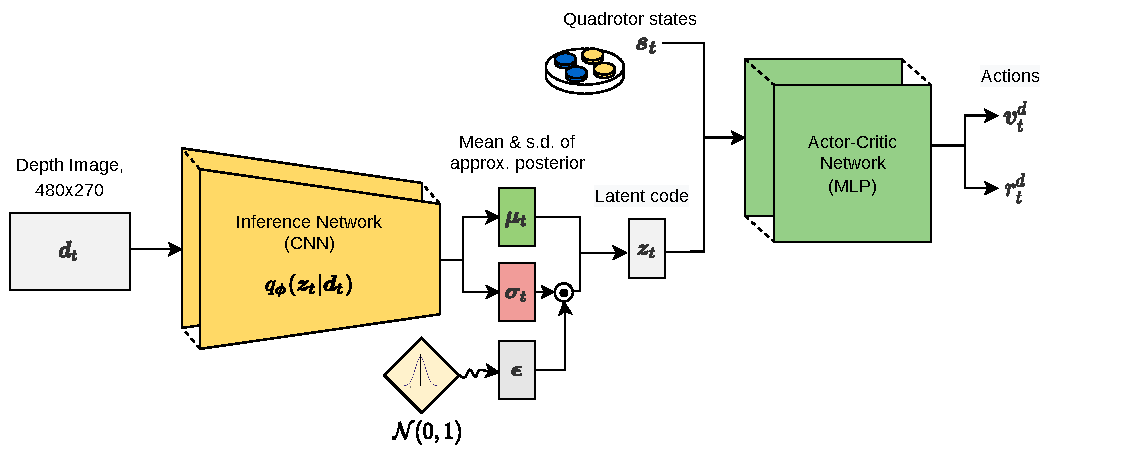
\includegraphics[width =1.1\textwidth]{figures/5_/5_overview.pdf}
    }
    \caption{An overview of our two-part model. The inference network (encoder) learns an approximate posterior distribution $\qzgived$, parametrised by a set of Gaussian distributions with an input-dependent mean $\boldsymbol{\mu}_t$ and diagonal covariance matrix $\boldsymbol{\sigma}_t$. We then sample this to get the latent representation $\z_t$. With $\s_t$ and $\z_t$, our agent -- a model-free actor-critic -- learns a policy $\actorpolicy$ which outputs a desired velocity $\v_t^d$ and yaw rate $r^d_t$.}
    \label{fig:5_overview}
\end{figure}

\section{Learning the Navigation Policy}
\label{sec:5_learning_navigation_policy}
Starting first with the navigation task, we solve the reinforcement learning problem through the use of PPO. Following the theory in \cref{subsec:2_PPO}, we aim to concurrently learn a critic value function $V_{\bt}(s)$ and actor policy $\pibtz$, parametrised with parameters $\bt$. To train our actor-critic for collision avoidance, we define a custom reward function and incorporate a \textit{curriculum} \cite{LearningWalkMassivelyParallel} during training.

\subsection{Reward Function}
\label{subsec:5_reward_function}
The reward function is one of the most powerful design tools within reinforcement learning. Using it to formalise the idea of a goal is also one of its most distinctive features \cite{suttonAndBartoBook}, since by deciding the reward structure of the environment, we can indirectly manipulate the learned agent behaviour to match the behaviour we hope to observe in testing. 
Though, for a navigational task, proper care must be taken to balance the rewards for different behaviours, such that an agent remains careful but also navigationally efficient. This is because the complex behaviour that an agent learns is based directly on the idea of maximising the total reward, which includes exploiting the environment and its reward function. Hence, any undesired behaviour that is observed during test time is often a consequence of a poorly designed reward function.

By weighing these considerations, we construct a reward function that builds on the implementation in \cite{IsaacGym}, but with additional rewards $R$ and penalties $P$ to shape the agent behaviour for collision avoidance.
First, we motivate the agent to minimise its distance to goal by rewarding its inverse distance to goal:
\begin{equation}
    \rew{pos} \, (S_t) = \frac{\gain{pos}}{1 + ||\p_t||_2}
\end{equation}
Then, we define a set of desired behaviours we wish to see when the agent is close to goal: remain still $\rew{vel}$, stay upright $\rew{up}$ and do not spin $\rew{spin}$:
\begin{align*}
    \rew{vel} \, (S_t) &= \frac{\gain{vel}}{1 + ||\v_t||_2} \numberthis \\[2mm]
    \rew{up} \, (S_t) &= \frac{\gain{up}}{1 + \left|1 - \mathcal{I}_z(\q_t)\right|^2}\,, \qquad 
    \mathcal{I}_z(\q_t) = \frac{\epsilon_2}{\sqrt{1-\eta^2}} \numberthis\\[2mm]
    \rew{spin} \, (S_t) &= \frac{\gain{spin}}{1 + r^2} \numberthis 
\end{align*}
Here, we use $\mathcal{I}_z(\q_t)$ to denote the upwards-ness of the quadrotor, where the idea is to represent the quadrotor orientation $\q_t$ in axis-angle form and then find the normalised $z$-component of the axis. For $\rew{spin}$, $r$ denotes the quadrotor yaw rate as shown in \eqref{eq:4_quadrotor_states_detailed}.

As for the conservative behaviour, we specify three penalties terms: one for velocities in the blind directions of the quadrotor (vertical and backward) $\pen{vel}$, one for being too close to an obstacle $\pen{depth}$, and the last for collision $\pen{collision}$:
\begin{align}
    \pen{vel} \, (S_t) &=  \alpha_{\text{vert}} \cdot w^2 + \alpha_{\text{back}} \cdot v_{\text{back}}^2 \, \qquad v_{\text{back}} = 
    \begin{cases} 
      v & \text{if} \; v \leq 0 \\
      0 & \text{else} 
   \end{cases} \\[2mm]
   \pen{depth} (S_t) &= \mu_{\text{dist}} \cdot \max \, \big(0, d_{\epsilon} - d_\text{obst}(S_t)\big)^2 \\[2mm]
  \pen{collision} (S_t) &= \begin{cases}
     \gain{collision} & \text{if} \; d_\text{obst}(S_t) \leq d_\text{collision} \\
     \gain{collision} & \text{if contact force detected} \\
     0 & \text{else}
  \end{cases}
\end{align}
The depth penalty $\pen{depth}$ is a simple one-sided quadratic barrier function taken from \cite{collision_free_MPC}, consisting of a scaling parameter $\mu_{\text{dist}}$ and safety margin $d_\epsilon$. Intuitively, this means that quadrotor receives no penalty if it is further than $d_\epsilon$, but is penalised an obstacle within $d_\epsilon$ is in sight. Thus, this should motivate the agent to stop moving closer to an obstacle, and to turn elsewhere. Visually, the depth penalty is shown in \cref{fig:5_depth_penalty}.
\begin{figure}[hbt]
    \centering
    \hspace{2cm}
    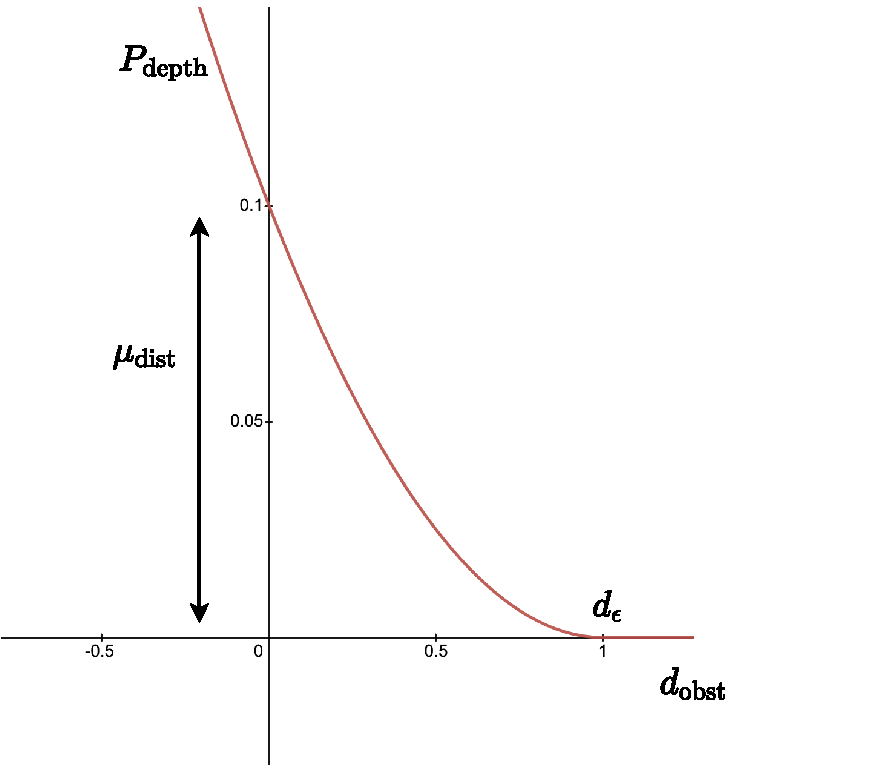
\includegraphics[width=0.6\textwidth]{figures/5_/5_depth_penalty.pdf}
    \caption{The depth penalty $\pen{depth}$ displaying the penalty for when an obstacle is closer than  $d_\epsilon = 1.0$m, when $\mu_{\text{dist}} = 0.1$. Diagram recreated from \cite{collision_free_MPC}.}
    \label{fig:5_depth_penalty}
\end{figure}

To find the distance to the closest obstacle $d_\text{obst}$, we project a point cloud from a depth image and take the norm of each point in the point cloud with the camera position and find the minimum. However, since we can only detect forward-facing collisions with the depth camera, we also detect collisions with a force sensor in simulation. 

From these, the full reward function is the sum of all rewards and penalties:
\begin{equation}
    R\,(S_t, \,A_t) = R_{\text{pos}} + R_{\text{pos}} \, (R_{\text{vel}} + R_{\text{up}} + R_{\text{spin}}) + P_{\text{vel}} + P_{\text{depth}} + P_{\text{collision}}
\end{equation}
where we specify $R_{\text{vel}}\,,\; R_{\text{up}}$ and $R_{\text{spin}}$ to only be important near goal by multiplying it with $\rew{pos}$.
Finally, the reward gains, penalty coefficients and distance parameters used for the reward function are listed in \cref{table:5_reward_parameters}.
\begin{table}[hbt]
    \renewcommand{\arraystretch}{1.0}
    \centering
    \begin{tabular}{||c|c||}
    \hline
    \centering
        Reward Parameter & Value \\ \hline \hline
        $\gain{pos}$ & 2.0 \\  
        $\gain{vel}$ & 1.0 \\ 
        $\gain{up}$ & 1.0 \\ 
        $\gain{spin}$ & 1.0 \\ 
        $\gain{collision}$ & -2 \\
        $\alpha_{\text{vert}}$ & -0.1 \\ 
        $\alpha_{\text{back}}$ & -0.01 \\ 
        $\mu_{\text{dist}}$ & -0.1 \\ 
        $d_{\text{collision}}$ & 0.2 \\ \hline
    \end{tabular}
    \caption{List of reward gains, penalty coefficients and distance parameters used in the reward function.}
     \label{table:5_reward_parameters}
\end{table}

We note that each of the reward terms are at maximum when $\p_t, \v_t = \boldsymbol{0}$, $r = 0$ and the quadrotor is upright. At this point, the quadrotor is directly on the goal, with a reward of $R_t^\text{max} = \gain{pos} + \gain{pos}(\gain{vel} + \gain{up} + \gain{spin}) = 8$ at every timestep, assuming that we avoid all penalties. However, when the quadrotor is very far from the goal, e.g. $>10$m, this goal-motivating reward begins to be very sparse. Combined with the conservative penalties, we can imagine that it will be difficult to train a policy end-to-end in a large cluttered environment due to negligible positive rewards for flying towards a goal and considerable negative rewards for going near obstacles.
This is also why we propose to use curriculum learning, which will be discussed in the next section.

\subsection{Curriculum Learning}
\label{subsec:5_curriculum}
The success of this thesis' approach can largely be attributed to the setup and procedure for training the reinforcement learning agent.
The term \textit{curriculum} was introduced by \cite{LearningWalkMassivelyParallel} and is used to describe the idea of training a policy at levels of increasing difficulty. For collision-free navigation, we leveraged this idea by training the quadrotor in progressively larger environments with an increasing density of obstacles. The reason for this can be justified by two reasons: first, training a randomly initialised policy in a very difficult environment with sparse rewards can be extremely time-consuming if not impossible; and second, collision avoidance is very generalisable -- once a quadrotor has learned to avoid one obstacle, it should not be difficult to extend this knowledge to two, and eventually many.

We assert that before a quadrotor can learn collision avoidance, it must first learn to fly towards the goal. Our primary concern is that reinforcement learning is generally considered sample-intensive, where learning a complicated policy may just come down to waiting for a lucky sequence of actions to be repeatedly executed. In this thesis, we aim to minimise this ``luck factor'' and instead propose a three-step process that should \textit{guarantee} successful training:
\begin{enumerate}
    \item First, learn to fly towards the goal with no obstacles present. 
    \item Then, learn basic obstacle avoidance by spawning the quadrotor and goal on opposite sides of \textit{one} obstacle, with the quadrotor facing the obstacle.
    \item Last, gradually increase the number of obstacles, the environment size and the episode length $T$ to obtain an advanced collision avoidance policy.
\end{enumerate}


\subsection{Network Architecture}
\label{subsec:5_MLP_architecture}
Moving on, the actor-critic network is chosen to be a shared three-layer MLP with two separate output heads: the policy head and the value function head. Its architecture is shown in \cref{fig:5_actor_critic}. The policy $\actorpolicy$ is modelled by the actor-network, which outputs a Gaussian distribution over actions for a given quadrotor state $\s_t$ and latent code $\z_t$. The value function is parametrised by the critic network that predicts the expected return (state value) for the same input.
\begin{figure}[hbt]
    \centering
    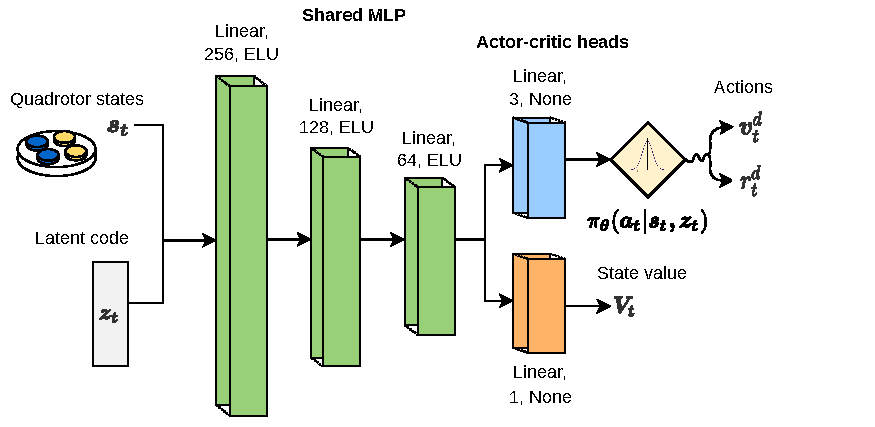
\includegraphics[width=0.9\textwidth]{figures/5_/5_actor_critic.pdf}
    \caption{The actor-critic network architecture. The actor and critic are parameterised by a shared base network comprised of a three-layer MLP with output dimensions $[256, 128, 64]$ and ELU activation functions, and two linear (fully-connected) output heads with linear activation functions. The actor parametrises a policy $\actorpolicy$ that outputs a Gaussian distribution over actions, while the critic parametrises a value function $\criticVF$ which predicts the expected return $V_t$.}
    \label{fig:5_actor_critic}
\end{figure}

\subsubsection{Shared Parameters in the Actor-Critic}
The concept behind using a shared structure in the actor-critic networks is that the \textit{base network} learns the \textit{features} our input so that these can be used by the \textit{network heads} for \textit{task-specific prediction or classification}. Essentially, it is the same as representation learning, where the last layer of the shared MLP contains the representation of features of the input. 
We can assume that in order to produce a correct velocity and yaw rate reference, the model should have some understanding of the agent-relative surroundings. Though in a similar vein, to be able to predict the expected return for a particular state requires the same understanding. So, in general, if two output tasks are largely related but utilise the same input, it makes sense to have a shared parametrisation for the base network with two task-specific heads.

\subsubsection{Size of the Network}
The size of the network was largely chosen according to other baseline models in \cite{IsaacGym}, and from previous experience from the project, thesis \cite{project_thesis}. From \cite{IsaacGym}, we noted that many examples utilise much larger networks, but these were also applied to tasks with ``more difficult'' observation-action mappings \cite{shadowHand, AMPMotionPriors} -- in essence, just having a much higher dimensional observation and action space.
This idea of using larger networks is that they have a larger \textit{generalisation potential}, thus enabling them to do well in more complicated tasks. Moreover, recent research also states that over-parametrization of neural networks might even be necessary to have robust results \cite{bubeck2021aLawOfRobustness}.
However, from experience in the project thesis, we found that larger networks take longer to train and do not necessarily produce better results immediately, therefore motivating a more conservative approach which is more in line with machine learning teachings: starting simple and increasing the complexity underway. From this, we found that a base network with size [256, 128, 64] was reasonable, along with 64 neurons for each head.

\subsubsection{Activation Functions}
In \cref{fig:5_actor_critic}, we note the use of two types of activation functions, the exponential linear unit (ELU) and linear (None), were most noteworthy is the choice of the linear activation function for the final network layer. Traditionally, we choose the final activation function based on the type of problem we have -- like \textit{sigmoid} for logistic regression (prediction or binomial classification tasks), or \textit{softmax} for multinomial logistic regression (multi-class classification). For continuous control problems with normalised action spaces, we often wish to limit our actions to a range of $[-1, 1]$, which actually makes \textit{tanh} the most suitable activation function. Nevertheless, the decision to use the linear activation function was large as a result of the baseline implementations in \cite{IsaacGym}. Instead, as an implementation detail, actions were left unbounded from the network but were clipped if their values exceeded $[-1, 1]$. 

Next, the exponential linear unit \cite{ELU} was also used due to being the default implementation in \cite{IsaacGym} -- with it also being used to solve other difficult tasks \cite{shadowHand, LearningWalkMassivelyParallel}. An alternative for MLPs is, of course, the widely popular rectified linear unit (ReLU) \cite{ReLU}, but the ELU differs slightly as it has negative values for inputs less than zero. This is shown more clearly in \eqref{eq:5_elu_activation} and \cref{fig:5_relu_elu}.
\begin{align}
        f_\text{ELU}(x) &= \begin{cases}
          x & \text{if} \; x > 0 \\
          \alpha \, (\exp{(x)} - 1) & \text{if} \; x \leq 0
        \end{cases}, \label{eq:5_elu_activation} \\
        f_\text{ReLU}(x) &= \begin{cases}
          x & \text{if} \; x > 0 \\
          0 & \text{if} \; x \leq 0
        \end{cases} \label{eq:5_relu_activation}
\end{align}
\begin{figure}[hbt]
    \centering
    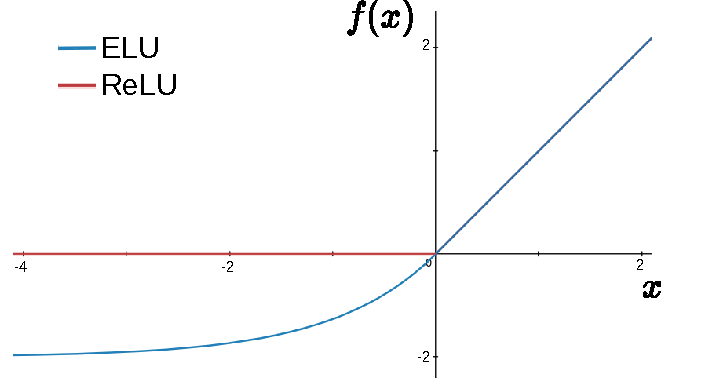
\includegraphics[width=0.5\textwidth]{figures/5_/5_relu_elu.pdf}
    \caption{Visualising the difference between the exponential linear unit (ELU) (with $\alpha = 1$) and rectified linear unit (ReLU) activation functions.}
    \label{fig:5_relu_elu}
\end{figure}

The primary reason for using ELU rather than ReLU is that one of the most significant problems of ReLU is that of \textit{dead neurons}. This problem occurs when a neuron is pushed to a negative weight (e.g. from a large update), because the gradient of the ReLU activation (its output) w.r.t the negative neuron weight will always be zero. To illustrate clearly, consider the perceptron $y = \text{ReLU}(Wx + b)$. When the a \textit{positive input} $x$ is multiplied with \textit{negative weights} $W$, the output $y$ is zero, and so too the gradient $\frac{\delta y}{\delta W}$. 
Conversely, if the \textit{input} $x$ and weights $W$ are \textit{negative}, the output $y$ is non-negative but the gradient of the output w.r.t the weights $\frac{\delta y}{\delta W} = \text{ReLU}' (x)$ is still zero because the ReLU gradient $\text{ReLU}'$ is zero for negative inputs.
As a result, the network weight will never be able to update itself as the gradient will be zero indefinitely, irrespective of the input data.
The benefit of ELU is that its gradient is non-zero for negative inputs close to zero. This helps to solve the \textit{dead-neuron problem} as it produces non-zero gradients that help to nudge network weights in the right direction, despite them having negative inputs. 

However, it can be argued that having some sparsity in the network (due to dead neurons) is actually an advantage, which is why ReLU is the default recommendation by \cite{DeepLearningBook} for modern neural networks and is also used in \cite{AMPMotionPriors} for its actor-critic MLP. Then again, too much sparsity can result in the network losing some of its generalisation capacity.

\section{Learning the Depth Representation}
\label{sec:5_learning_representation}
To tackle the unsupervised representation learning problem, we use a convolutional VAE to learn the latent representation for the depth data $\d$. We use the method presented by \cite{variational_bayes} for optimising the VAE, whose theory is outlined in \cref{subsec:2_VAE_variational_autoencoders}. Additionally, to both deal with the constrained dimension of the latent space and make our VAE suitable for collision avoidance, we introduce a custom loss function that allows us to specify which depth characteristics the VAE should prioritise in its reconstructions and choose a lightweight network architecture inspired from \cite{deepCollisionPredictorOracle}, and \cite{vae_decoder_architecture}.

\subsection{Ideal Depth Reconstruction With a Customised Reconstruction Loss}
\label{subsec:5_vae_reconstruction}
We first recall that the \textit{reconstruction loss} in \eqref{eq:2_vae_loss_estimator_single_datapoint} defines the learned behaviour of our generative network $\pdgivez$. In a vanilla VAE, it defines that the decoder $\pdgivez$ should learn to reconstruct $\d_t$ from $\z_t$, where $\z_t$ is the sampled latent code from our encoder $\qzgived$ for a given $\d_t$. Now, the key insight is that in order to properly reconstruct $\d_t$, any features of $\d_t$ that should be reconstructed must be present in $\z_t$ -- from which the VAE learned to do through the joint optimisation of the encoder and decoder in \eqref{eq:2_vae_loss_estimator_dataset}.
This implies that if we define certain features of $\d_t$ to be more costly than others, their loss will be over-represented in the reconstruction loss, and the VAE would prioritise learning these in its latent space so that these specific features could be reconstructed, and the VAE loss minimised. 

Thus, our approach is to \textit{alter the reconstruction loss} such that the VAE learns which features of the depth image distribution to prioritise in its latent space. With this, we attempt to prioritise the features in \cref{sec:4_representation_learning_task} in the latent space by presenting the following modifications:
\begin{enumerate}
    \item \textbf{Filtered targets} -- Instead of using the input $\d_t$ as the target reconstructions of our generative model $\pdgivez$, we use a filtered depth image $\d^f$ as the target. This means that for a given depth image $\d_t$, the generative network instead learns a probability distribution $\pdfgivezt$, where $\d^f_t = f(\d_t)$ is given by a deterministic filtering process $f$ of the depth image $\d_t$, and $\z_t \sim \qzgived$ is the sampled latent code from our encoder with input $\d_t$.
    \item \textbf{Depth weighting} -- We weigh the pixel-wise reconstruction error by a function of its observed depth. This means that the reconstruction error for pixels showing close obstacles in $\d^f_t$ are weighed more than pixels of far obstacles.
    \item \textbf{Added edge loss} -- We add the an additional mean-absolute error (MAE) term to the reconstruction error of filtered-obstacle edge pixels.
\end{enumerate}

To go more in detail, the filtering process is the IP-Basic algorithm \cite{filtering_depth_completion} for dilation and hole closing, as used in \cite{LearningStateRepresentation} and \cite{deepCollisionPredictorOracle}. Its implementation is a result of a few benefits for our task. First, minimising the complexity of depth images by rounding shapes emphasises only learning rough shapes. Also, as dilation increases obstacle sizes, filtering provides an extra layer of safety regarding collision avoidance. Finally, filtering also removes noise, which can be important when testing this framework on a real robotic system.
Then, to avoid the extra computational load of pre-filtering depth images on the robot, we use filtered images as reconstruction targets for some depth input, such that the VAE learns to implicitly perform the filtering process in its forward-pass \cite{LearningStateRepresentation}.

As for the depth weighting, we multiply the pixel-wise error of a reconstruction with the bounded depth gain $K_{\text{depth}}(d_{i,j})$, a function of the filtered-depth pixel value $d_{i,j}$:
\begin{equation}
    K_{\text{depth}}(d_{i,j}) = \alpha_\text{depth} \cdot \min \Bigg(\frac{1}{d_{i,j} + 0.5}, 1\Bigg) \qquad \text{for} \quad  i, j \in \dim \, (\d_t^f)
    \label{eq:5_depth_gain}
\end{equation}
which is illustrated in \cref{fig:5_depth_gain}.
\begin{figure}[hbt]
    \centering
    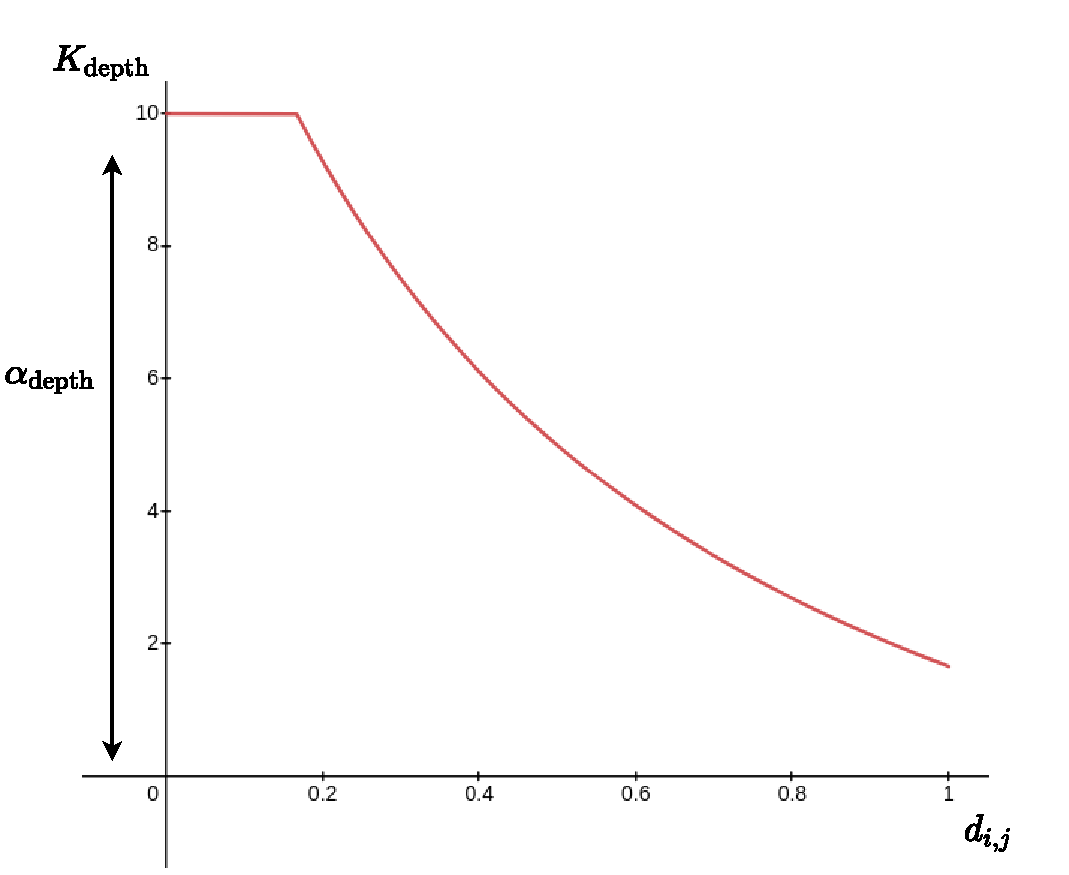
\includegraphics[width=0.5\textwidth]{figures/5_/5_depth_gain.pdf}
    \caption{The depth gain to weigh the pixel-wise reconstruction error. Reconstruction errors for very close obstacles (pixel values $d_{i,j}<0.16$) are weighed the same, with $\alpha_\text{depth} = 10.0$.}
    \label{fig:5_depth_gain}
\end{figure}
The idea for the depth weighting is that if we increase the reconstruction error according to its closeness, the pixel-wise loss of close obstacles should dominate the pixel-wise loss of obstacles far away. So close obstacles should be prioritised in the latent space representation.
Intuitively, this is particularly important for collision avoidance: we wish to distinguish between pixel-wise errors for obstacles far away compared to those immediately nearby. For example, a 1m error for an obstacle 7m away should be considered less important than the same as a 1m error for an obstacle 1.5m away.

We also see that thin obstacles are expected to be reconstructed when they are close by combining depth weighting with filtered targets. This is because their reconstruction targets are more prominent, as many more pixels will produce a high loss, particularly at close range.

Finally, we used a simple homemade procedure to implement the added edge loss. First, we used a Canny edge detector \cite{canny_edge_detection} to find the obstacle edges in $\d_t^f$. After, we used a Gaussian filter to dilate the edges -- taking any pixel value over 0 as an edge. Finally, the pixel-wise MAE of filtered depth reconstruction was multiplied by this image-edge mask to achieve the edge loss. Since we motivated this for clearer reconstructions, the Gaussian filter had to be used to dilate the edges of the image-edge mask. This is because, for the MAE loss to account for the object's shape, it is essential to add the pixel-wise error along the edges of obstacles and the pixel-wise error of neighbouring pixels. 


\subsection{Network Architecture}
\label{subsec:5_vae_architecture}
With the loss function covered, what remains is the architecture of the VAE. As mentioned, our VAE design was mainly inspired by the work of \cite{deepCollisionPredictorOracle} and \cite{vae_decoder_architecture}, where we utilise a convolution-based encoder-decoder structure.
The overall structure of the VAE is shown in \cref{fig:5_vae} and its parameters are detailed in \cref{app:vae_params}.
\begin{figure}[hbt]
    \centering
    \makebox[\textwidth]{
        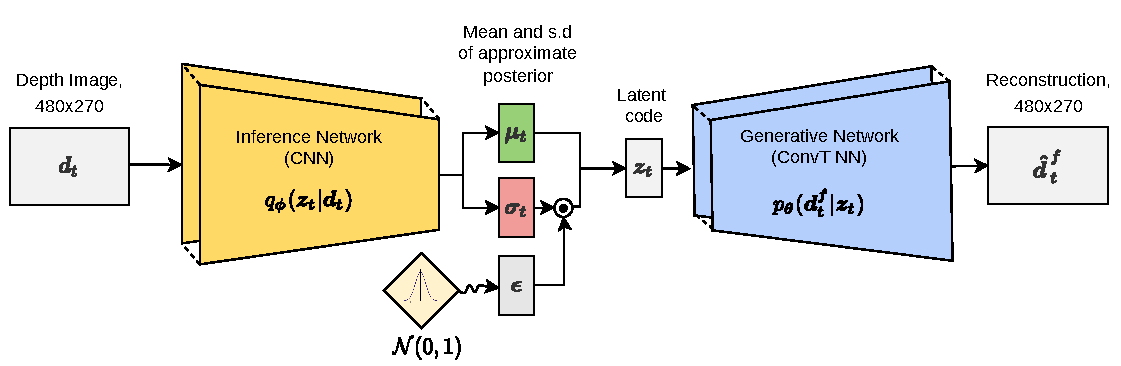
\includegraphics[width=\textwidth]{figures/5_/5_vae.pdf}}
    \caption{The VAE network architecture. The encoder is parametrised by a CNN, while the encoder is parametrised by a transposed CNN (ConvT NN). Given a depth image $\d_t$, we can sample from the inference network $\qzgived$ to obtain a latent code $\z_t$. The generative network $\pdfgivez$ then learns to construct the filtered depth image $\d^f_t = f(\d_t)$ from the latent code$\z_t$.}
    \label{fig:5_vae}
\end{figure}

\subsubsection{Inference Network}
\label{subsubsec:5_vae_inference_network}
Our encoder is follows the CNN design of \cite{deepCollisionPredictorOracle}, though utilises instead two convolution layers before a ResNet8 \cite{KaimingResNet}, with two fully-connected layers at the end. Its structure is shown in \cref{fig:5_encoder}, while the residual blocks are depicted in \cref{fig:5_res_block}.
\begin{figure}[H]
    \centering
        \makebox[\textwidth]{
        \hspace{1mm}
        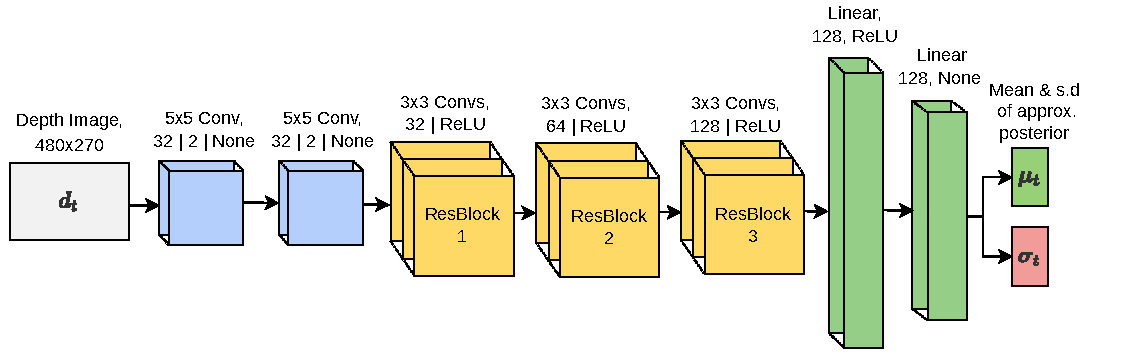
\includegraphics[width=1.\textwidth]{figures/5_/5_encoder.pdf}
    }
    \caption{The encoder network architecture. It comprises two convolution layers, with 32 $5\times5$ filters with a stride of 2, three residual blocks with $[32, 64, 128]$ output filters, and two fully connected layers with output dimensions $[128, 128]$. The dimension of the feature map is (roughly) halved for each convolution layer and residual block due to the 2-strided convolutions. The size of the feature map after the last convolution is $15\times9$. (See \cref{app:vae_encoder} for details)}
    \label{fig:5_encoder}
\end{figure}
\begin{figure}[H]
    \centering
    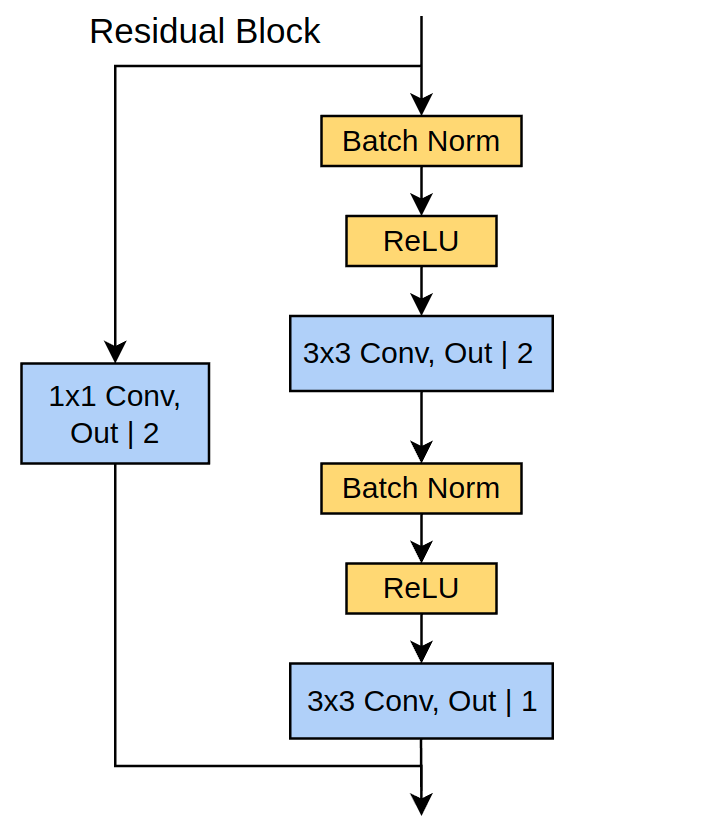
\includegraphics[width=0.4\textwidth]{figures/5_/5_res_block.png}
    \caption{The residual block architecture. A convolution by a $1\times1$ filter (kernel), with stride 2 is applied to the shortcut connection. $Out$ represents the number of filters of the residual block.}
    \label{fig:5_res_block}
\end{figure}
Regarding our design choices, these were primarily motivated by two factors -- we desired a lightweight network and wished to reduce the dimension of the feature map to be small enough but not too small. 
The ResNet8 was suitable to satisfy the first aspect, while the depth of the network (through stridden convolutions) was decided to satisfy the other. We also found during testing that reducing the feature dimension below $15 \times 9$ (to $8 \times 5$) resulted in a much worse reconstruction output, discouraging the use of another residual block or stridden convolution layer.
However, this choice resulted in a dramatically sized linear layer that accounted for 86\% of the encoder weights -- ($128 \cdot 15\times9) \cdot 128$ connections.
Nevertheless, this was unavoidable since 128 was the minimum number of neurons in the linear layer (64 means and log-variances), which left the alternatives: to either reduce the feature dimension or the number of filters. Though, both options were tested and did not improve results, leaving the conclusion that this is a feature and not a disadvantage of our encoder.


\subsubsection{Generative Network}
\label{subsubsec:5_vae_generative_network}
The generative network is inspired from \cite{vae_decoder_architecture}, with an additional linear layer and transposed convolution layer. Its architecture is shown in \cref{fig:5_decoder}. 
\begin{figure}[hbt]
    \centering
        \makebox[\textwidth]{
        \hspace{1mm}
        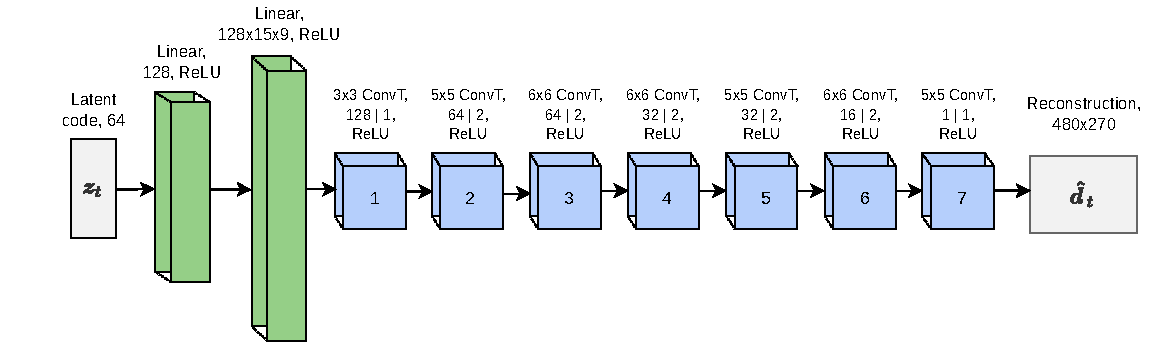
\includegraphics[width=\textwidth]{figures/5_/5_decoder.pdf}
    }
    \caption{The decoder network architecture comprises two linear layers and seven transposed convolution layers. Each strode transposed convolution roughly the dimension of the feature map to achieve the final dimension feature map dimension $480\times270$. (See \cref{app:vae_decoder} for details)}
    \label{fig:5_decoder}
\end{figure}
The primary design rule for autoencoders is that the decoder should be a mirror of the encoder so that the network resembles an \textit{hourglass}. As a result, we followed the encoder with two linear layers, including the large linear layer that connects 128 neurons to 128, $9\times5$ filters. As for the transposed convolutions, this is a relatively simple but effective design. The only design choice here was the filter size and number of filters, though these were chosen primarily to match the layer-wise feature dimensions of the encoder and their overall sizes.

Vigorous testing was also done with a ResNet8 decoder, which was designed to mirror our encoder. However, despite its more advanced structure -- with batch normalisation and shortcut connections -- no significant performance gain was observed in training. Conversely, checkerboard artefacts and divergence in training were often observed when training on the whole dataset due to uncertain reasons, though it could be to the layer-wise stacking of stridden transposed convolutions with identical filter dimensions \cite{odena2016deconvolution}. Therefore, a final decision was made to use the decoder in \cref{fig:5_decoder}.
\chapter{Proposed Approach}
\label{chap:5_proposed_approach}

This chapter presents the methodology for solving the autonomous navigation task outlined in the previous chapter. Overall, we propose a CNN-MLP model where, given a depth image $\d_t$ and the quadrotor states $\s_t$, it decides a continuous velocity $\v^d_t$ and steering $r^d_t$ command that should avoid obstacles in a cluttered environment, while travelling towards some goal in 3-dimensional space.
We will present and discuss this two-part model's design choices, starting with the MLP module for learning the navigation policy, then later the encoder-decoder-based CNN inference network used for representation learning. An overview of the model is shown in \cref{fig:5_overview}.
\begin{figure}[hbt]
    \centering
    \makebox[\textwidth]{
        \hspace{15mm}
        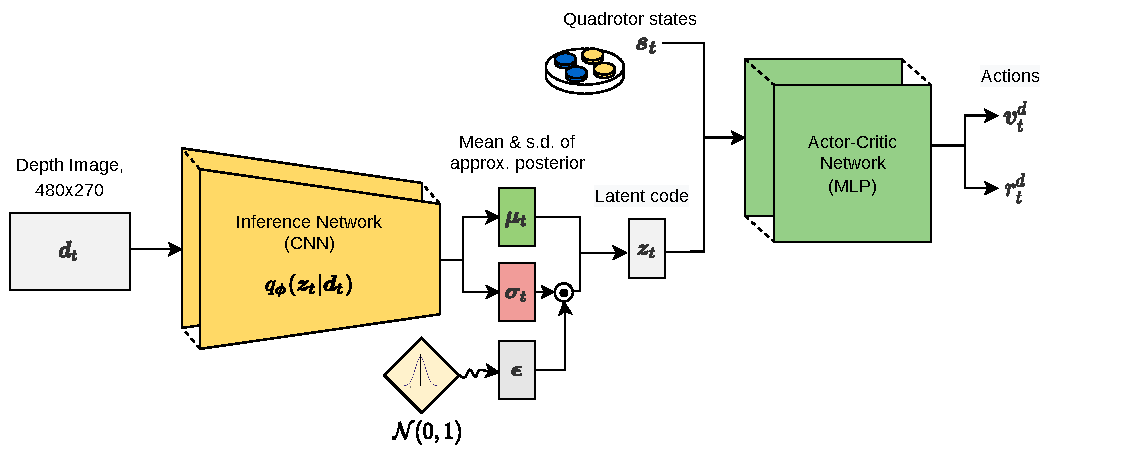
\includegraphics[width =1.1\textwidth]{figures/5_/5_overview.pdf}
    }
    \caption{An overview of our two-part model. The inference network (encoder) learns an approximate posterior distribution $\qzgived$, parametrised by a set of Gaussian distributions with an input-dependent mean $\boldsymbol{\mu}_t$ and diagonal covariance matrix $\boldsymbol{\sigma}_t$. We then sample this to get the latent representation $\z_t$. With $\s_t$ and $\z_t$, our agent -- a model-free actor-critic -- learns a policy $\actorpolicy$ which outputs a desired velocity $\v_t^d$ and yaw rate $r^d_t$.}
    \label{fig:5_overview}
\end{figure}

\section{Learning the Navigation Policy}
\label{sec:5_learning_navigation_policy}
Starting first with the navigation task, we solve the reinforcement learning problem through the use of PPO. Following the theory in \cref{subsec:2_PPO}, we aim to concurrently learn a critic value function $V_{\bt}(s)$ and actor policy $\pibtz$, parametrised with parameters $\bt$. To train our actor-critic for collision avoidance, we define a custom reward function and incorporate a \textit{curriculum} \cite{LearningWalkMassivelyParallel} during training.

\subsection{Reward Function}
\label{subsec:5_reward_function}
The reward function is one of the most powerful design tools within reinforcement learning. Using it to formalise the idea of a goal is also one of its most distinctive features \cite{suttonAndBartoBook}, since by deciding the reward structure of the environment, we can indirectly manipulate the learned agent behaviour to match the behaviour we hope to observe in testing. 
For a navigational task, proper care must be taken to balance the rewards for different behaviours, so an agent remains navigationally efficient but careful. This is because the complex behaviour that an agent learns is based directly on the idea of maximising the total reward, which includes exploiting the environment and its reward function. Hence, any undesired behaviour that is observed during test time is often a consequence of a poorly designed reward function.

By weighing these considerations, we construct a reward function that builds on the implementation in \cite{IsaacGym}, but with additional rewards $R$ and penalties $P$ to shape the agent behaviour for collision avoidance.
First, we motivate the agent to minimise its distance to goal by rewarding its inverse distance to goal:
\begin{equation}
    \rew{pos} \, (S_t) = \frac{\gain{pos}}{1 + ||\p_t||_2}
\end{equation}
Then, we define a set of desired behaviours we wish to see when the agent is close to goal: remain still $\rew{vel}$, stay upright $\rew{up}$ and do not spin $\rew{spin}$:
\begin{align*}
    \rew{vel} \, (S_t) &= \frac{\gain{vel}}{1 + ||\v_t||_2} \numberthis \\[2mm]
    \rew{up} \, (S_t) &= \frac{\gain{up}}{1 + \left|1 - \mathcal{I}_z(\q_t)\right|^2}\,, \qquad 
    \mathcal{I}_z(\q_t) = \frac{\epsilon_2}{\sqrt{1-\eta^2}} \numberthis\\[2mm]
    \rew{spin} \, (S_t) &= \frac{\gain{spin}}{1 + r^2} \numberthis 
\end{align*}
Here, we use $\mathcal{I}_z(\q_t)$ to denote the upwards-ness of the quadrotor, where the idea is to represent the quadrotor orientation $\q_t$ in axis-angle form and then find the normalised $z$-component of the axis. For $\rew{spin}$, $r$ denotes the quadrotor yaw rate as shown in \eqref{eq:4_quadrotor_states_detailed}.

As for the conservative behaviour, we specify three penalties terms: one for velocities in the blind directions of the quadrotor (vertical and backward) $\pen{vel}$, one for being too close to an obstacle $\pen{depth}$, and the last for collision $\pen{collision}$:
\begin{align}
    \pen{vel} \, (S_t) &=  \alpha_{\text{vert}} \cdot w^2 + \alpha_{\text{back}} \cdot v_{\text{back}}^2 \, \qquad v_{\text{back}} = 
    \begin{cases} 
      v & \text{if} \; v \leq 0 \\
      0 & \text{else} 
   \end{cases} \\[2mm]
   \pen{depth} (S_t) &= \mu_{\text{dist}} \cdot \max \, \big(0, d_{\epsilon} - d_\text{obst}(S_t)\big)^2 \\[2mm]
  \pen{collision} (S_t) &= \begin{cases}
     \gain{collision} & \text{if} \; d_\text{obst}(S_t) \leq d_\text{collision} \\
     \gain{collision} & \text{if contact force detected} \\
     0 & \text{else}
  \end{cases}
\end{align}
The depth penalty $\pen{depth}$ is a simple one-sided quadratic barrier function taken from \cite{collision_free_MPC}, consisting of a scaling parameter $\mu_{\text{dist}}$ and safety margin $d_\epsilon$. Intuitively, this means that quadrotor receives no penalty if it is further than $d_\epsilon$, but is penalised an obstacle within $d_\epsilon$ is in sight. Thus, this should motivate the agent to stop moving closer to an obstacle, and to turn elsewhere. Visually, the depth penalty is shown in \cref{fig:5_depth_penalty}.
\begin{figure}[hbt]
    \centering
    \hspace{2cm}
    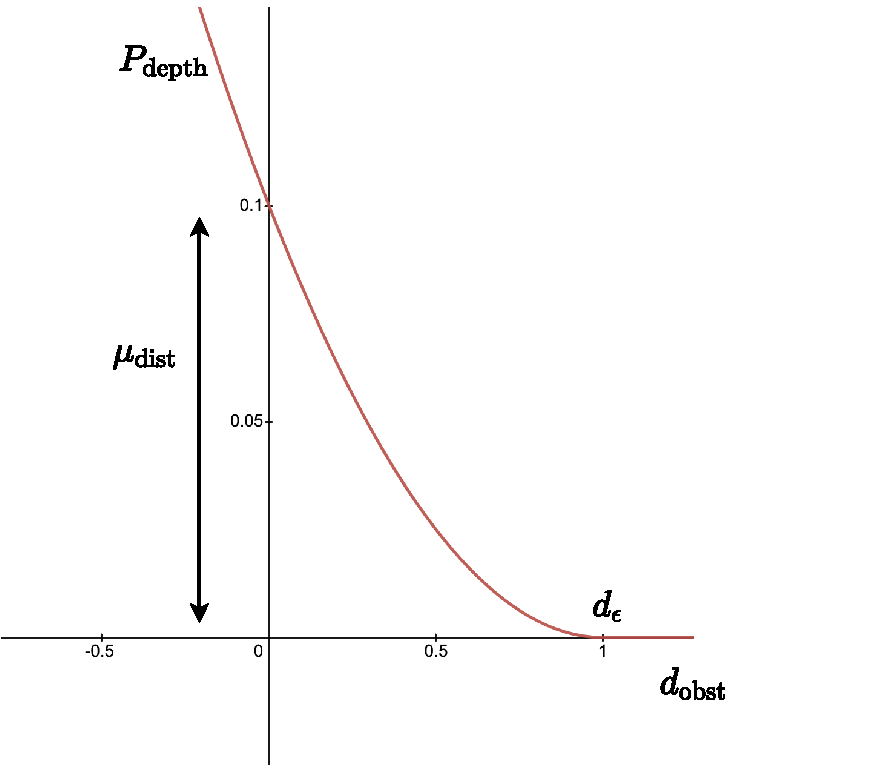
\includegraphics[width=0.6\textwidth]{figures/5_/5_depth_penalty.pdf}
    \caption{The depth penalty $\pen{depth}$ displaying the penalty for when an obstacle is closer than  $d_\epsilon = 1.0$m, when $\mu_{\text{dist}} = 0.1$. Diagram recreated from \cite{collision_free_MPC}.}
    \label{fig:5_depth_penalty}
\end{figure}

To find the distance to the closest obstacle $d_\text{obst}$, we project a point cloud from a depth image and take the norm of each point in the point cloud with the camera position and find the minimum. However, since we can only detect forward-facing collisions with the depth camera, we also detect collisions with a force sensor in simulation. 

From these, the full reward function is the sum of all rewards and penalties:
\begin{equation}
    R\,(S_t, \,A_t) = R_{\text{pos}} + R_{\text{pos}} \, (R_{\text{vel}} + R_{\text{up}} + R_{\text{spin}}) + P_{\text{vel}} + P_{\text{depth}} + P_{\text{collision}}
\end{equation}
where we specify $R_{\text{vel}}\,,\; R_{\text{up}}$ and $R_{\text{spin}}$ to only be important near goal by multiplying it with $\rew{pos}$.
Finally, the reward gains, penalty coefficients and distance parameters used for the reward function are listed in \cref{table:5_reward_parameters}.
\begin{table}[hbt]
    \renewcommand{\arraystretch}{1.0}
    \centering
    \begin{tabular}{||c|c||}
    \hline
    \centering
        Reward Parameter & Value \\ \hline \hline
        $\gain{pos}$ & 2.0 \\  
        $\gain{vel}$ & 1.0 \\ 
        $\gain{up}$ & 1.0 \\ 
        $\gain{spin}$ & 1.0 \\ 
        $\gain{collision}$ & -2 \\
        $\alpha_{\text{vert}}$ & -0.1 \\ 
        $\alpha_{\text{back}}$ & -0.01 \\ 
        $\mu_{\text{dist}}$ & -0.1 \\ 
        $d_{\text{collision}}$ & 0.2 \\ \hline
    \end{tabular}
    \caption{List of reward gains, penalty coefficients and distance parameters used in the reward function.}
     \label{table:5_reward_parameters}
\end{table}

We note that each of the reward terms are at maximum when $\p_t, \v_t = \boldsymbol{0}$, $r = 0$ and the quadrotor is upright. At this point, the quadrotor is directly on the goal, with a reward of $R_t^\text{max} = \gain{pos} + \gain{pos}(\gain{vel} + \gain{up} + \gain{spin}) = 8$ at every timestep, assuming that we avoid all penalties. However, when the quadrotor is very far from the goal, e.g. $>10$m, this goal-motivating reward begins to be very sparse. Combined with the conservative penalties, we can imagine that it will be difficult to train a policy end-to-end in a large cluttered environment due to negligible positive rewards for flying towards a goal and considerable negative rewards for going near obstacles.
This is also why we propose to use curriculum learning, which will be discussed in the next section.

\subsection{Curriculum Learning}
\label{subsec:5_curriculum}
The success of this thesis' approach can largely be attributed to the setup and procedure for training the reinforcement learning agent.
The term \textit{curriculum} was introduced by \cite{LearningWalkMassivelyParallel} and is used to describe the idea of training a policy at levels of increasing difficulty. For collision-free navigation, we leveraged this idea by training the quadrotor in progressively larger environments with an increasing density of obstacles. Two reasons can justify the reason for this: first, training a randomly initialised policy in a very difficult environment with sparse rewards can be highly time-consuming if not impossible; and second, collision avoidance is very generalisable -- once a quadrotor has learned to avoid one obstacle, it should not be difficult to extend this knowledge to two, and eventually many.

We assert that before a quadrotor can learn collision avoidance, it must first learn to fly towards the goal. Our primary concern is that reinforcement learning is generally considered sample-intensive. Learning a complicated policy may just come down to waiting for a lucky sequence of actions to be repeatedly executed. In this thesis, we aim to minimise this ``luck factor'' and instead propose a three-step process that should \textit{guarantee} successful training:
\begin{enumerate}
    \item First, learn to fly towards the goal with no obstacles present. 
    \item Then, learn basic obstacle avoidance by spawning the quadrotor and goal on opposite sides of \textit{one} obstacle, with the quadrotor facing the obstacle.
    \item Last, gradually increase the number of obstacles, the environment size and the episode length $T$ to obtain an advanced collision avoidance policy.
\end{enumerate}


\subsection{Network Architecture}
\label{subsec:5_MLP_architecture}
Moving on, the actor-critic network is chosen to be a shared three-layer MLP with two separate output heads: the policy head and the value function head. Its architecture is shown in \cref{fig:5_actor_critic}. The policy $\actorpolicy$ is modelled by the actor-network, which outputs a Gaussian distribution over actions for a given quadrotor state $\s_t$ and latent code $\z_t$. The value function is parametrised by the critic network that predicts the expected return (state value) for the same input.
\begin{figure}[hbt]
    \centering
    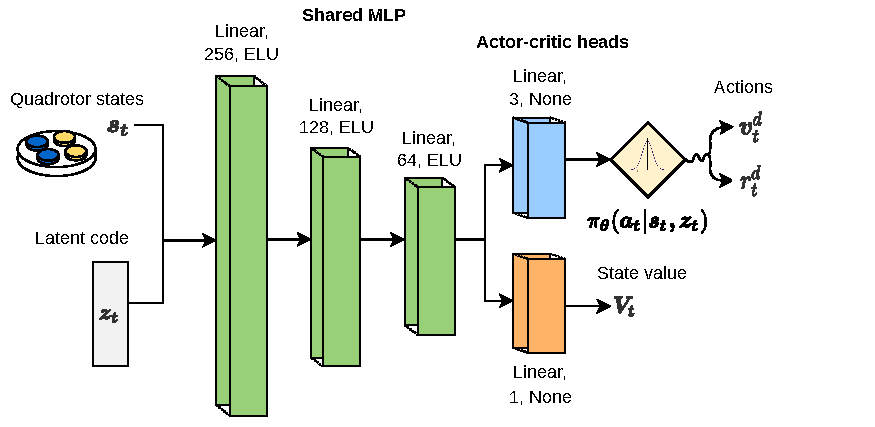
\includegraphics[width=0.9\textwidth]{figures/5_/5_actor_critic.pdf}
    \caption{The actor-critic network architecture. The actor and critic are parameterised by a shared base network comprised of a three-layer MLP with output dimensions $[256, 128, 64]$ and ELU activation functions, and two linear (fully-connected) output heads with linear activation functions. The actor parametrises a policy $\actorpolicy$ that outputs a Gaussian distribution over actions, while the critic parametrises a value function $\criticVF$ which predicts the expected return $V_t$.}
    \label{fig:5_actor_critic}
\end{figure}

\subsubsection{Shared Parameters in the Actor-Critic}
The concept behind using a shared structure in the actor-critic networks is that the \textit{base network} learns the \textit{features} our input so that these can be used by the \textit{network heads} for \textit{task-specific prediction or classification}. Essentially, it is the same as representation learning, where the last layer of the shared MLP contains the representation of features of the input. 
We can assume that to produce a correct velocity and yaw rate reference, the model should have some understanding of the agent-relative surroundings. Though in a similar vein, to be able to predict the expected return for a particular state requires the same understanding. So, in general, if two output tasks are largely related but utilise the same input, it makes sense to have a shared parametrisation for the base network with two task-specific heads.

\subsubsection{Size of the Network}
The size of the network was largely chosen according to other baseline models in \cite{IsaacGym}, and from previous experience from the project, thesis \cite{project_thesis}. From \cite{IsaacGym}, we noted that many examples utilise much larger networks, but these were also applied to tasks with ``more difficult'' observation-action mappings \cite{shadowHand, AMPMotionPriors} -- in essence, just having a much higher dimensional observation and action space.
This idea of using larger networks is that they have a larger \textit{generalisation potential}, thus enabling them to do well in more complicated tasks. Moreover, recent research also states that over-parametrization of neural networks might even be necessary to have robust results \cite{bubeck2021aLawOfRobustness}.
However, from experience in the project thesis, we found that larger networks take longer to train and do not necessarily produce better results immediately, therefore motivating a more conservative approach which is more in line with machine learning teachings: starting simple and increasing the complexity underway. From this, we found that a base network with size [256, 128, 64] was reasonable, along with 64 neurons for each head.

\subsubsection{Activation Functions}
In \cref{fig:5_actor_critic}, we note the use of two types of activation functions, the exponential linear unit (ELU) and linear (None), were most noteworthy is the choice of the linear activation function for the final network layer. Traditionally, we choose the final activation function based on the type of problem we have -- like \textit{sigmoid} for logistic regression (prediction or binomial classification tasks), or \textit{softmax} for multinomial logistic regression (multi-class classification). For continuous control problems with normalised action spaces, we often wish to limit our actions to a range of $[-1, 1]$, which actually makes \textit{tanh} the most suitable activation function. Nevertheless, the decision to use the linear activation function was large as a result of the baseline implementations in \cite{IsaacGym}. Instead, as an implementation detail, actions were left unbounded from the network but were clipped if their values exceeded $[-1, 1]$. 

Next, the exponential linear unit \cite{ELU} was also used due to being the default implementation in \cite{IsaacGym} -- with it also being used to solve other difficult tasks \cite{shadowHand, LearningWalkMassivelyParallel}. An alternative for MLPs is, of course, the widely popular rectified linear unit (ReLU) \cite{ReLU}, but the ELU differs slightly as it has negative values for inputs less than zero. This is shown more clearly in \eqref{eq:5_elu_activation} and \cref{fig:5_relu_elu}.
\begin{align}
        f_\text{ELU}(x) &= \begin{cases}
          x & \text{if} \; x > 0 \\
          \alpha \, (\exp{(x)} - 1) & \text{if} \; x \leq 0
        \end{cases}, \label{eq:5_elu_activation} \\
        f_\text{ReLU}(x) &= \begin{cases}
          x & \text{if} \; x > 0 \\
          0 & \text{if} \; x \leq 0
        \end{cases} \label{eq:5_relu_activation}
\end{align}
\begin{figure}[hbt]
    \centering
    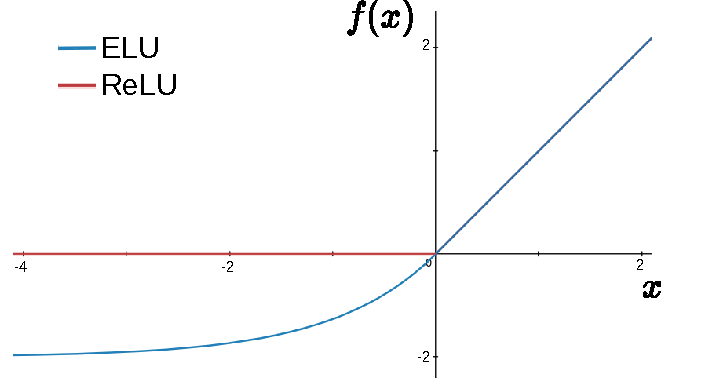
\includegraphics[width=0.5\textwidth]{figures/5_/5_relu_elu.pdf}
    \caption{Visualising the difference between the exponential linear unit (ELU) (with $\alpha = 1$) and rectified linear unit (ReLU) activation functions.}
    \label{fig:5_relu_elu}
\end{figure}

The primary reason for using ELU rather than ReLU is that one of the most significant problems of ReLU is that of \textit{dead neurons}. This problem occurs when a neuron is pushed to a negative weight (e.g. from a large update), because the gradient of the ReLU activation (its output) w.r.t the negative neuron weight will always be zero. To illustrate clearly, consider the perceptron $y = \text{ReLU}(Wx + b)$. When the a \textit{positive input} $x$ is multiplied with \textit{negative weights} $W$, the output $y$ is zero, and so too the gradient $\frac{\delta y}{\delta W}$. 
Conversely, if the \textit{input} $x$ and weights $W$ are \textit{negative}, the output $y$ is non-negative but the gradient of the output w.r.t the weights $\frac{\delta y}{\delta W} = \text{ReLU}' (x)$ is still zero because the ReLU gradient $\text{ReLU}'$ is zero for negative inputs.
As a result, the network weight will never be able to update itself as the gradient will be zero indefinitely, irrespective of the input data.
The benefit of ELU is that its gradient is non-zero for negative inputs close to zero. This helps to solve the \textit{dead-neuron problem} as it produces non-zero gradients that help to nudge network weights in the right direction, despite them having negative inputs. \todo{maybe move to theory}

However, it can be argued that having some sparsity in the network (due to dead neurons) is actually an advantage, which is why ReLU is the default recommendation by \cite{DeepLearningBook} for modern neural networks and is also used in \cite{AMPMotionPriors} for its actor-critic MLP. Then again, too much sparsity can result in the network losing some of its generalisation capacity.

\section{Learning the Depth Representation}
\label{sec:5_learning_representation}
To tackle the unsupervised representation learning problem, we use a convolutional VAE to learn the latent representation for the depth data $\d$. We use the method presented by \cite{variational_bayes} for optimising the VAE, whose theory is outlined in \cref{subsec:2_VAE_variational_autoencoders}. Additionally, to both deal with the constrained dimension of the latent space and make our VAE suitable for collision avoidance, we introduce a custom loss function that allows us to specify which depth characteristics the VAE should prioritise in its reconstructions and choose a lightweight network architecture inspired from \cite{deepCollisionPredictorOracle}, and \cite{vae_decoder_architecture}.

\subsection{Ideal Depth Reconstruction With a Customised Reconstruction Loss}
\label{subsec:5_vae_reconstruction}
We first recall that the \textit{reconstruction loss} in \eqref{eq:2_vae_loss_estimator_single_datapoint} defines the learned behaviour of our generative network $\pdgivez$. In a vanilla VAE, it defines that the decoder $\pdgivez$ should learn to reconstruct $\d_t$ from $\z_t$, where $\z_t$ is the sampled latent code from our encoder $\qzgived$ for a given $\d_t$. Now, the key insight is that in order to properly reconstruct $\d_t$, any features of $\d_t$ that should be reconstructed must be present in $\z_t$ -- from which the VAE learned to do through the joint optimisation of the encoder and decoder in \eqref{eq:2_vae_loss_estimator_dataset}.
This implies that if we define certain features of $\d_t$ to be more costly than others, their loss will be over-represented in the reconstruction loss, and the VAE would prioritise learning these in its latent space so that these specific features could be reconstructed, and the VAE loss minimised. 

Thus, our approach is to \textit{alter the reconstruction loss} such that the VAE learns which features of the depth image distribution to prioritise in its latent space. With this, we attempt to prioritise the features in \cref{sec:4_representation_learning_task} in the latent space by presenting the following modifications:
\begin{enumerate}
    \item \textbf{Filtered targets} -- Instead of using the input $\d_t$ as the target reconstructions of our generative model $\pdgivez$, we use a filtered depth image $\d^f$ as the target. This means that for a given depth image $\d_t$, the generative network instead learns a probability distribution $\pdfgivezt$, where $\d^f_t = f(\d_t)$ is given by a deterministic filtering process $f$ of the depth image $\d_t$, and $\z_t \sim \qzgived$ is the sampled latent code from our encoder with input $\d_t$.
    \item \textbf{Depth weighting} -- We weigh the pixel-wise reconstruction error by a function of its observed depth. This means that the reconstruction error for pixels showing close obstacles in $\d^f_t$ are weighed more than pixels of far obstacles.
    \item \textbf{Added edge loss} -- We add the an additional mean-absolute error (MAE) term to the reconstruction error of filtered-obstacle edge pixels.
\end{enumerate}

To go more in detail, the filtering process is the IP-Basic algorithm \cite{filtering_depth_completion} for dilation and hole closing, as used in \cite{LearningStateRepresentation} and \cite{deepCollisionPredictorOracle}. Its implementation is a result of a few benefits for our task. First, minimising the complexity of depth images by rounding shapes emphasises only learning rough shapes. Also, as dilation increases obstacle sizes, filtering provides an extra layer of safety regarding collision avoidance. Finally, filtering also removes noise, which can be important when testing this framework on a real robotic system.
Then, to avoid the extra computational load of pre-filtering depth images on the robot, we use filtered images as reconstruction targets for some depth input, such that the VAE learns to implicitly perform the filtering process in its forward-pass \cite{LearningStateRepresentation}.

As for the depth weighting, we multiply the pixel-wise error of a reconstruction with the bounded depth gain $K_{\text{depth}}(d_{i,j})$, a function of the filtered-depth pixel value $d_{i,j}$:
\begin{equation}
    K_{\text{depth}}(d_{i,j}) = \alpha_\text{depth} \cdot \min \Bigg(\frac{1}{d_{i,j} + 0.5}, 1\Bigg) \qquad \text{for} \quad  i, j \in \dim \, (\d_t^f)
\end{equation}
which is illustrated in \cref{fig:5_depth_gain}.
\begin{figure}[hbt]
    \centering
    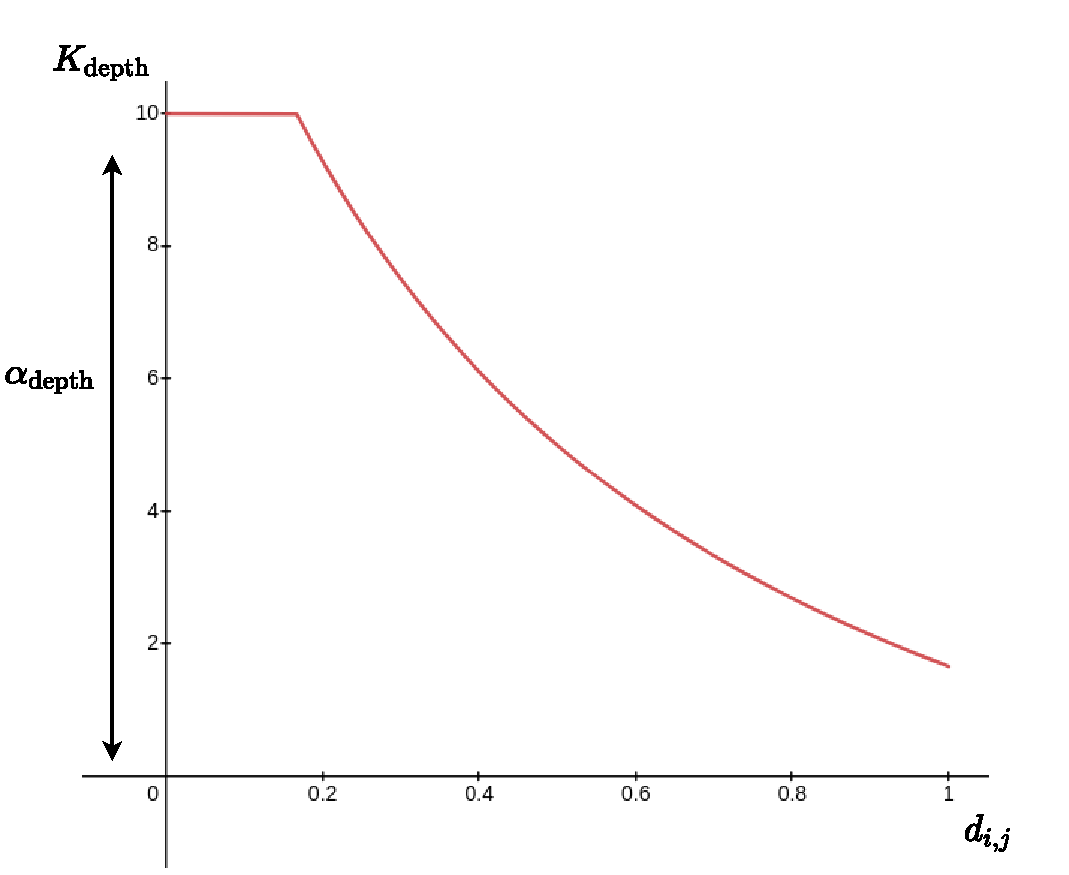
\includegraphics[width=0.5\textwidth]{figures/5_/5_depth_gain.pdf}
    \caption{The depth gain to weigh the pixel-wise reconstruction error. Reconstruction errors for very close obstacles (pixel values $d_{i,j}<0.16$) are weighed the same, with $\alpha_\text{depth} = 10.0$.}
    \label{fig:5_depth_gain}
\end{figure}
The idea for the depth weighting is that if we increase the reconstruction error according to its closeness, the pixel-wise loss of close obstacles should dominate the pixel-wise loss of obstacles far away. So close obstacles should be prioritised in the latent space representation.
Intuitively, this is particularly important for collision avoidance: we wish to distinguish between pixel-wise errors for obstacles far away compared to those immediately nearby. For example, a 1m error for an obstacle 7m away should be considered less important than the same as a 1m error for an obstacle 1.5m away.

We also see that thin obstacles are expected to be reconstructed when they are close by combining depth weighting with filtered targets. This is because their reconstruction targets are more prominent, as many more pixels will produce a high loss, particularly at close range.

Finally, we used a simple homemade procedure to implement the added edge loss. First, we used a Canny edge detector \cite{canny_edge_detection} to find the obstacle edges in $\d_t^f$. After, we used a Gaussian filter to dilate the edges -- taking any pixel value over 0 as an edge. Finally, the pixel-wise MAE of filtered depth reconstruction was multiplied by this image-edge mask to achieve the edge loss. Since we motivated this for clearer reconstructions, the Gaussian filter had to be used to dilate the edges of the image-edge mask. This is because, for the MAE loss to account for the object's shape, it is essential to add the pixel-wise error along the edges of obstacles and the pixel-wise error of neighbouring pixels. 


\subsection{Network Architecture}
\label{subsec:5_vae_architecture}
With the loss function covered, what remains is the architecture of the VAE. As mentioned, our VAE design was mainly inspired by the work of \cite{deepCollisionPredictorOracle} and \cite{vae_decoder_architecture}, where we utilise a convolution-based encoder-decoder structure.
The overall structure of the VAE is shown in \cref{fig:5_vae} and its parameters are detailed in \cref{app:vae_params}.
\begin{figure}[hbt]
    \centering
    \makebox[\textwidth]{
        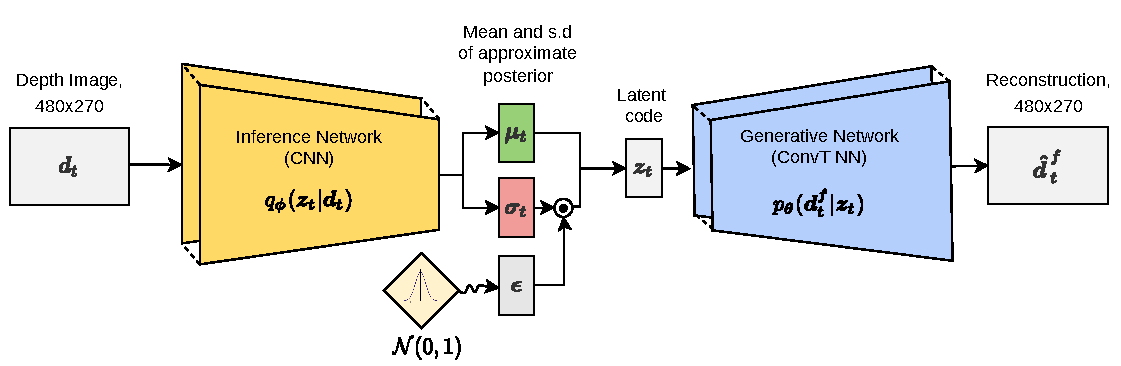
\includegraphics[width=\textwidth]{figures/5_/5_vae.pdf}}
    \caption{The VAE network architecture. The encoder is parametrised by a CNN, while the encoder is parametrised by a transposed CNN (ConvT NN). Given a depth image $\d_t$, we can sample from the inference network $\qzgived$ to obtain a latent code $\z_t$. The generative network $\pdfgivez$ then learns to construct the filtered depth image $\d^f_t = f(\d_t)$ from the latent code$\z_t$.}
    \label{fig:5_vae}
\end{figure}

\subsubsection{Inference Network}
\label{subsubsec:5_vae_inference_network}
Our encoder is follows the CNN design of \cite{deepCollisionPredictorOracle}, though utilises instead two convolution layers before a ResNet8 \cite{KaimingResNet}, with two fully-connected layers at the end. Its structure is shown in \cref{fig:5_encoder}, while the residual blocks are depicted in \cref{fig:5_res_block}.
\begin{figure}[H]
    \centering
        \makebox[\textwidth]{
        \hspace{1mm}
        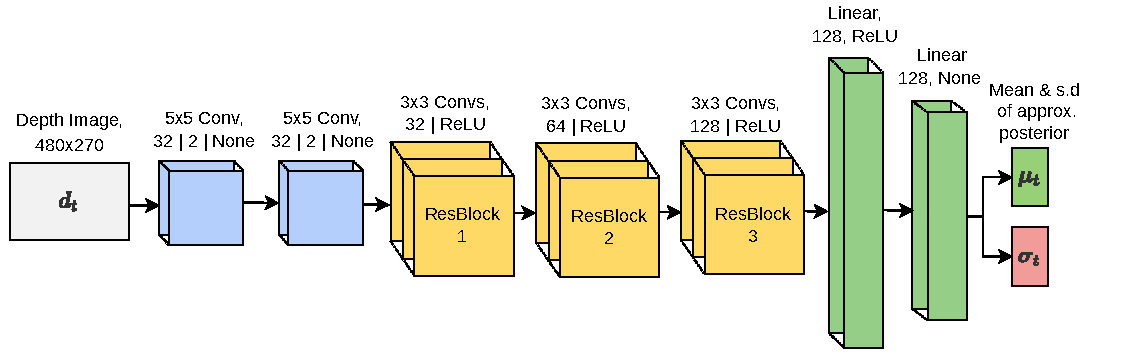
\includegraphics[width=1.\textwidth]{figures/5_/5_encoder.pdf}
    }
    \caption{The encoder network architecture. It comprises two convolution layers, with 32 $5\times5$ filters with a stride of 2, three residual blocks with $[32, 64, 128]$ output filters, and two fully connected layers with output dimensions $[128, 128]$. The dimension of the feature map is (roughly) halved for each convolution layer and residual block due to the 2-strided convolutions. The size of the feature map after the last convolution is $15\times9$. (See \cref{app:vae_encoder} for details)}
    \label{fig:5_encoder}
\end{figure}
\begin{figure}[H]
    \centering
    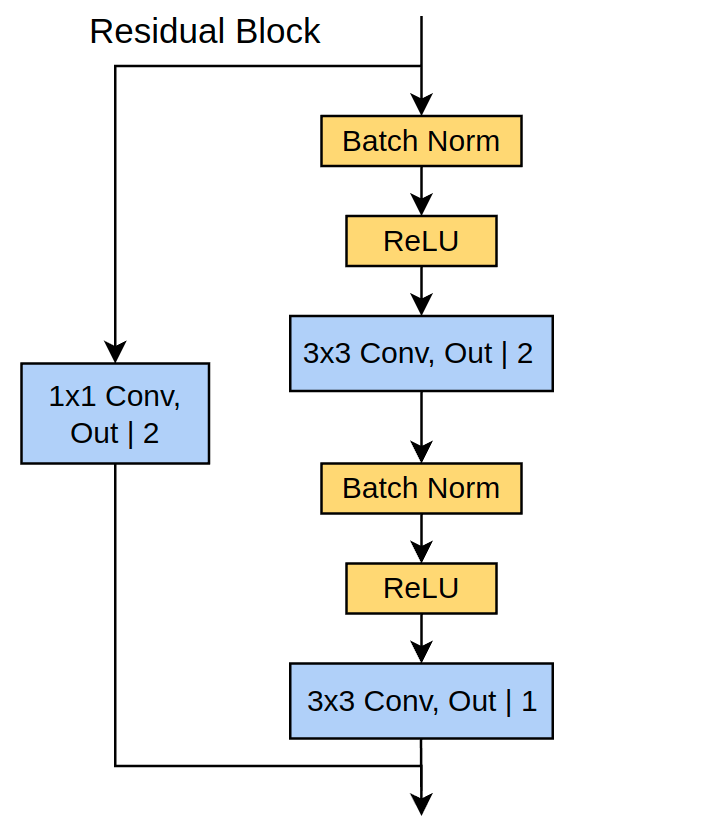
\includegraphics[width=0.4\textwidth]{figures/5_/5_res_block.png}
    \caption{The residual block architecture. A convolution by a $1\times1$ filter (kernel), with stride 2 is applied to the shortcut connection. $Out$ represents the number of filters of the residual block.}
    \label{fig:5_res_block}
\end{figure}
Regarding our design choices, these were primarily motivated by two factors -- we desired a lightweight network and wished to reduce the dimension of the feature map to be small enough but not too small. 
The ResNet8 was suitable to satisfy the first aspect, while the depth of the network (through stridden convolutions) was decided to satisfy the other. We also found during testing that reducing the feature dimension below $15 \times 9$ (to $8 \times 5$) resulted in a much worse reconstruction output, discouraging the use of another residual block or stridden convolution layer.
However, this choice resulted in a dramatically sized linear layer that accounted for 86\% of the encoder weights -- ($128 \cdot 15\times9) \cdot 128$ connections.
Nevertheless, this was unavoidable since 128 was the minimum number of neurons in the linear layer (64 means and log-variances), which left the alternatives: to either reduce the feature dimension or the number of filters. Though, both options were tested and did not improve results, concluding that this is a feature and not a disadvantage of our encoder.


\subsubsection{Generative Network}
\label{subsubsec:5_vae_generative_network}
The generative network is inspired from \cite{vae_decoder_architecture}, with an additional linear layer and transposed convolution layer. Its architecture is shown in \cref{fig:5_decoder}. 
\begin{figure}[hbt]
    \centering
        \makebox[\textwidth]{
        \hspace{1mm}
        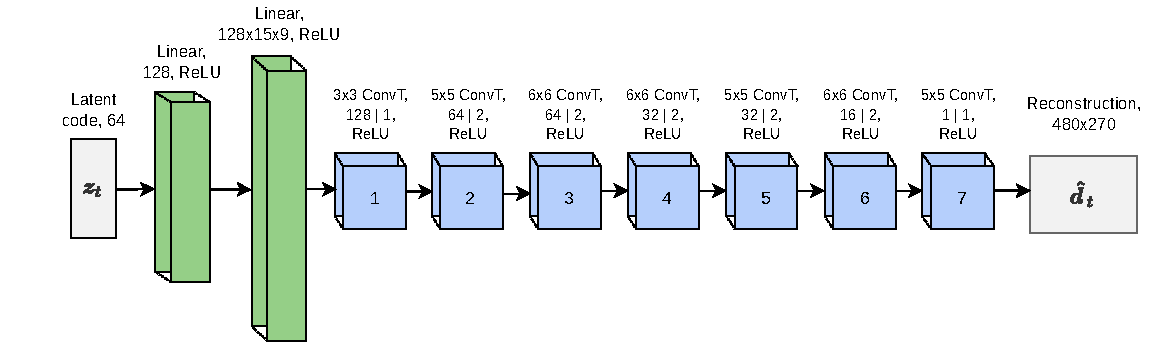
\includegraphics[width=\textwidth]{figures/5_/5_decoder.pdf}
    }
    \caption{The decoder network architecture comprises two linear layers and seven transposed convolution layers. Each strode transposed convolution roughly the dimension of the feature map to achieve the final dimension feature map dimension $480\times270$. (See \cref{app:vae_decoder} for details)}
    \label{fig:5_decoder}
\end{figure}
The primary design rule for autoencoders is that the decoder should be a mirror of the encoder so that the network resembles an \textit{hourglass}. As a result, we followed the encoder with two linear layers, including the large linear layer that connects 128 neurons to 128, $9\times5$ filters. As for the transposed convolutions, this is a relatively simple but effective design. The only design choice here was the filter size and number of filters, though these were chosen primarily to match the layer-wise feature dimensions of the encoder and their overall sizes.

Vigorous testing was also done with a ResNet8 decoder, which was designed to mirror our encoder. However, despite its more advanced structure -- with batch normalisation and shortcut connections --, no significant performance gain was observed in training. Conversely, divergence in training was often observed when training on the whole dataset for unknown reasons. Therefore, a final decision was made to use the decoder in \cref{fig:5_decoder}.
\chapter{Navigation Policy Evaluation Studies}
\label{chap:7_navigation_policy_evaluation_studies}

\begin{comment}
Evaluation without Obstacles
Evaluation with sparse obstacles out of the way
Evaluation when obstacle avoidance is necessary
\end{comment}


For our thesis, training and simulation was done on an Intel(R) Core(TM) i9-10940X CPU @ 3.30GHz desktop PC, with three NVIDIA GeForce RTX 3090 GPUs. 

\section{Policy Performance along the Learning Curriculum}
Put table here

\subsection{Without Obstacles}
\subsection{1 Obstacles}
\subsection{3 Obstacles}
\subsection{5 Obstacles}
\subsection{9 Obstacles}

\section{Evaluating the Learned Navigation Policy}

Test in 3 ``hard'' envs

For each
2-3 qualitative results (maps, path, actions vel ref)
statistical study with randomized  - numbers of times it crashes

\subsection{Known Obstacles}

\subsection{New Obstacles}

\subsection{New Environment}
\chapter{VAE Evaluation Studies}
\label{chap:8_vae_evaluation_studies}
\chapter{Discussion}
\label{chap:9_discussion}

\section{Navigation Policy}
When and why does unsupervised pretraining work, chap 15.1.1 book
unsupervised pretraining is likely to be most useful when the function to be learned is extremely complicated. \cite{DeepLearningBook}

Read discussion from \cite{pfeiffer2017perception}. Very good points and at the end:
``Furthermore, we observed that the deep planner is able to avoid small dead ends if it approaches them from the outside. Once the robot enters a convex dead-end region, it is not capable of freeing itself. In addition to that, the robot’s heading sometimes fluctuates before avoiding an obstacle. This issue will be further analyzed and might be solved by using recurrent neural networks with internal memory''. We have the same exact issue -- purely reactionary.

It has often been assumed that standard policy search methods such as those explored in the present
work are simply too fragile to scale to difficult problems: End-to-End Training of Deep Visuomotor Policies paper, very relevant start.

Standard policy search is thought to be difficult because it deals simultaneously with complex environmental dynamics and a complex police, cite DDPG.

Autonomous Drone Racing with PPO \cite{song2021droneRacing}, they said 3 reasons for success: stable and fast training through 1) parallel sampling scheme 2) distributed initialisation strategy 3) random track curriculum. Gate poses are sent as observations

Simultaneously, there has also been developments in GPU-based differentiable physics simulators, making it possible to calculate the analytic gradients and make efficient use of it when finding the policy gradient \cite{oldDifferentiablePhysicsSimulator, differentiablePhysicsSimulator}. Could lead to faster learning. 

\cite{MotionPlanningAmongDynamicAgentsDRL2018} states that pretraining is necessary for them, otherwise robot wanders around and never accumulates reward (in 3C). After pretrainig, reaches goal every time, but poor for collision avoidance.

Standard model-free deep RL aims to unify these challenges of representation learning and task learning into a single end-to-end training procedure. However, solving both problems together is difficult, since an effective policy requires an effective representation, and an effective representation requires meaningful gradient information to come from the policy or value function, while using only the model-free supervision signal (i.e., the reward function). As a result, learning directly from images with standard end-to-end RL algorithms can in practice be slow, sensitive to hyperparameters, and inefficient. SLAC \cite{stochastic_latent_actor_critic} intro. Opposite of navrep \cite{NavRep_unsupervised}.

NavRep paper also found that only marginal performance was gained in using LSTM hidden state, most important was to include z encoding from VAE (page 6).

For example, if the reward function is overcompensating for conservative behaviour -- such as a large reward for being far from obstacles -- this expectation could well be met but through the agent remaining completely still.
 
The overall initial concern is that reinforcement learning is generally sample-intensive, which is why learning a policy from scratch almost always demands the use of a simulator. For complicated tasks, it can be difficult to learn the policy unless the policy repeatedly attempts ``lucky'' sequences of actions which provide a high reward and large gradient to push the network in the right direction. Having an observation space with dimension $\R^{77}$ means that a lot of numbers are changing and for an agent -- imperative to first know which is important for goal-reaching.
 
warmStart (training a network with pre-existing weights) is generally bad -- paper from Microsoft \cite{warmStart}. Empirical study. Particularly for recommender systems, when you have input streams, how should you update your model? combine new date with old and retrain (cold-start)? or combine new with old and from existing weights (warm-start)? Cold-start always performs better unintuitively. \cite{warmStart} shrink-and-perturb trick (half weights and add gaussian noise) is best. I guess strictly speaking we don't have new data, it is the same? but in new environments I guess you can classify it as new data -- so possible technique to try out.
 
Parallel initialisation -- where do I put this? So I think one of the main reasons why project failed is explained abstractly in batch-size invariance paper \cite{batchsizeInvariance}. Basically, when performing gradient updates, the update rule in TRPO \eqref{eq:2_trpo_actor_objective} is based on off-policy importance sampling -- because behaviour policy is not the same as update policy, we compensate (remove bias) by weighing gradient updates by the ratio. However, look at decoupled policy objective in \cite{batchsizeInvariance}, one of the reasons for stability is that updated policy has to stay close to prox policy -- by close we mean not similar to behaviour policy, but how \textit{old} prox policy is. When doing updates, two choices for choosing pi old when calculating the ratio: the policy immediately preceding the current iteration, pi recent, and the behaviour policy pi behav. For project, when we got high gradients, pi old became very old after many iterations (8 updates from 8000 batch steps), so new policy unstable. Instead, gradients should be weighted by how different they from policy used to collect data. 
Isaac gym -- we are allowed to use big batch sizes, because parallel means that big batch still only has few steps and updates often. when doing updates, the trajectory is always filled with experience from recent policy. check this though

One of the main conclusions in \cite{project_thesis} is that due to the limited exploratory nature of on-policy PPO, a parallel initialisation scheme would be very beneficial to help prevent the agent from converging to some local optimum. This is also why \cite{song2021droneRacing} credits a parallel initialisation scheme as one of three key factors for success.


\section{VAE}
mobilenetv3-small is used in high-speed flight in the wild (instead of DroNet) has 224x3 default input size with 2.5 mil params. 

Random initialisation -- symmetry breaking \cite{LectureNotesSparseAutoencoder}.

See appendix B in VAE paper \cite{variational_bayes}. The analytic solution for KL divergence between approx posterior and prior is introduced, but the implementation in train\_vae.py was missing a .pow(2) on logvar -- saw the same in other implementations. Keras tutorial loss doesn't use analytic solution, instead just computes log of Gaussian pdfs and takes the difference (same as KL div), works well.

often we want batch norm for stability, KL div already pushes latent variables to follow normal distribution, so this is a nice side-effect during training.


binary cross-entropy does maximum likeihood estimatiion, but it assumes our data is Bernoulli distributed (black white pixels) -- pushes pixels to either 0 or 1.
MSE is maximum likelihood estimation, which is cross entropy too, but it assumes our target distribution $p(\d)$ is Gaussian. That's why it is centered around 0.5.
remember that we're minimising the KL divergence between our input data and model. VAEs specify a regularisation term that penalises p-z from deviating from Gaussian, but it does not make an assumption on p-data. This is specified in the reconstruction loss.
\chapter{Conclusions}
\label{chap:10_conclusions}
\begin{comment}
A concise summary of essential information and findings in the project.
\end{comment}

Learning-based approaches to autonomous navigation in cluttered environments are becoming increasingly popular due to being able to learn flexible, complex behaviours that can solve a variety of challenging tasks, without the need to explicitly program them. Due to their ability to represent complex functions through deep architectures, they are able to direct map raw sensor inputs to actions which, combined with the fast parallel computing hardware, allows them to plan and execute actions at a speed in at which a model-based pipeline cannot compete.
Further, when presented with a novel task with no prior demonstrations and an an optimal solution that is hard to formulate, reinforcement learning provides a method to learn this through only the specification of an abstract reward function.

In this this thesis, we thus explored the ability of reinforcement learning to solve a collision avoidance task for a quadrotor, using only a depth camera. We proposed the use of a two part CNN-MLP model, where the CNN is the inference network of the VAE, while the MLP served as the reinforcement learning agent actor-critic. To shape our model for collision avoidance, we then introduced a novel reward function for the reinforcement learning agent, and a novel loss function for the VAE. The reward function was shaped with penalties to demotivate risky behaviour, which in hindsight may have not been optimal due to the inherent sparsity of rewards. Similarly, the customised reconstruction error of the VAE enabled us to prioritise collision-relevant features of depth images, though potentially resulted in over-fitting of the depth data distribution.

Nonetheless, the evaluation studies showed that the overall approach was successful at its task, achieving 98.6\% in the hard environment which accounted for tight space. The approach also showed a promising robustness to noise, where its adverse effects were most present in tight paths, such as in the hard environment. Despite these results, the study also showed that much could improved, both in the proposed approach and the implementation of our model. Specifically, it was shown that many pass-by collisions occur due to blindness when turning, the agent frequently reversed or descended into collisions, and the agent maintained a bias when navigating past obstacles.
It was discussed that to alleviate these problems, the concept of an internal memory had to be added to the policy, through for example the hidden state of an RNN, such that the agent is capable of predicting collisions more than one timesteps ahead, remembering passed obstacles, and finally capable of deciding more fine-tuned actions which account for these. Otherwise, implementation errors included a too small margin between the goal height and ground, a lack of normalisation in the environment setup. 

On the VAE side, we saw that the \todo{finish}

\section{Further Work}
\label{sec:10_further_work}

train across a wider variety of environments, and number of obstacles and size at the same time.

No linearised dynamics in simulator for quadrotor. 
Have a proper quadrotor model. 
test with unseen obstacles.
add LSTM or transformer.

more ablation studies?

compare navigation results using other VAE models

Simultaneously, there has also been developments in GPU-based differentiable physics simulators, making it possible to calculate the analytic gradients and make efficient use of it when finding the policy gradient \cite{oldDifferentiablePhysicsSimulator, differentiablePhysicsSimulator}. Could lead to faster learning. 


\printbibliography
\appendix
\chapter{Algorithms}
\label{app:algs}

\section{One-step Actor-Critic}
\label{app:algs_ActorCritic}
\begin{algorithm}
\caption{One-step Actor-Critic, from \cite{suttonAndBartoBook}} \label{alg:OneStepActorCritic}
    \begin{algorithmic}[1]
    \State Input: a differentiable policy parameterisation $\pi (a \mid s, \boldsymbol{\theta}$
    \State Input: a differentiable state-value function parameterisation $\hat{v}(s, \boldsymbol{w})$
    \State Parameters: step sizes $\alpha^{\boldsymbol{\theta}} > 0$, $\alpha^{\boldsymbol{w}} > 0$ (learning rates)
    \State Initialize policy parameters $\boldsymbol{\theta} \in \R^{d'}$ and state-value weights $\boldsymbol{w} \in \R^d$
    \For {each episode}
    
        \State Initialize S (first state of episode)
        \State I $\gets$ 1
        
        \While {\text{S is not terminal}}
        
            \State A $\sim \pi ( \dot \mid S, \boldsymbol{\theta})$
            \State Take action A, observe S', R
            \State $\delta \leftarrow R + \gamma \hat{v}(S', \boldsymbol{w}) - \hat{v}(S, \boldsymbol{w})$
            \State $\boldsymbol{w} \leftarrow \boldsymbol{w} + \alpha^{\boldsymbol{w}} \delta \nabla \hat{v}(S, \boldsymbol{w})$
            \State $\boldsymbol{\theta} \leftarrow \boldsymbol{\theta} + \alpha^{\boldsymbol{\theta}} I \delta \nabla \ln \pi (A \mid S, \boldsymbol{\theta})$
            \State $I \leftarrow \gamma I$
            \State $S \leftarrow S'$
        \EndWhile
    \EndFor
    \end{algorithmic}
\end{algorithm}
\noindent
This implementation is taken from the Sutton \& Barto's book \cite{suttonAndBartoBook}.

\newpage
\section{Proximal Policy Optimization}
\label{app:algs_PPO}

\begin{algorithm}
\caption{PPO Actor-Critic style, from \cite{PPO}} \label{alg:PPO_actorCriticStyle}
\begin{algorithmic}[1]
\For {iteration = 1, 2, ...}
    \For{actor = 1, 2, ..., $N$}
        \State Run policy $\pi_{\theta_{old}}$ in environment for $T$ timesteps
        \State Compute advantage estimates $\hat{A}_1 ,..., \hat{A}_T$
    \EndFor
    
    \State Optimize surrogate L with respect to $\theta$, with K epochs and minibatch size $M \leq NT$
    \State $\theta_{old} \leftarrow \theta $
\EndFor
\end{algorithmic}
\end{algorithm}
\noindent
This implementation is acquired from the original paper \cite{PPO}. Note that in our implementation we have $N=512$ actors. \vspace{8mm}

\begin{algorithm}
\caption{PPO-Clip, from \href{https://spinningup.openai.com/en/latest/algorithms/ppo.html}{Spinning Up, OpenAI}} \label{alg:PPO_spinningUp}
\begin{algorithmic}[1]
\State Input: initial policy parameters $\theta_0$, initial value function parameters $\phi_0$
\For {k = 0, 1, 2, ...}
    \State Collect set of trajectories $\mathcal{D}_k = \{\tau_i\}$ by running policy $\pi_k = \pi(\theta_k)$ in the environment.
    \State Compute the return $\hat{R}_t$.
    \State Compute advantage estimates, $\hat{A}_t$ based on the current value function $V_{\phi_k}$
    \State Update the policy by maximizing the PPO-Clip objective:
    \[
    \theta_{k+1} = \arg \max_\theta \frac{1}{|\mathcal{D}_k|T} \sum_{\tau \in \mathcal{D}_k} \sum^{T}_{t=0} \min \left(
    \frac{\pi_\theta (a_t | s_t)}{\pi_{\theta_k} (a_t | s_t)} 
    A^{\pi_{\theta_k}}(s_t, \, a_t), \,\, g(\epsilon, A^{\pi_{\theta_k}}(s_t, \, a_t))
    \right),
    \]
    typically via a stochastic gradient ascent algorithm with Adam.
    \State Fit value function by regression on mean-squared error:
    \[
    \phi_{k+1} = \arg \min_\phi \frac{1}{|\mathcal{D}_k|T} \sum_{\tau \in \mathcal{D}_k} \sum^{T}_{t=0}
    \Big(
    V_\phi (s_t) - \hat{R}_t
    \Big)^2,
    \]
    typically via some stochastic gradient descent algorithm.
\EndFor
\end{algorithmic}
\end{algorithm}

\noindent
Algorithm \ref{alg:PPO_spinningUp} is acquired from OpenAI's Spinning Up documentation:\\
https://spinningup.openai.com/en/latest/algorithms/ppo.html 

\newpage
\section{Auto-Encoding Variational Bayes}
\label{app:algs_vae}

\begin{algorithm}
\caption{Minibatch version of Auto-Encoding Variational Bayes (AEVB) algorithm, from \cite{variational_bayes}} \label{alg:vae_variational_bayes}
\begin{algorithmic}[2]
\State $\bt, \boldsymbol{\phi} \leftarrow$ Initialise parameters
\Repeat
    \State $\boldsymbol{X}^M \leftarrow$ Random minibatch of $M$ datapoints (drawn from the full dataset)
    \State $\boldsymbol{\epsilon} \leftarrow$ random samples from noise distribution $p(\boldsymbol{\epsilon})$
    \State $\boldsymbol{g} \leftarrow \nabla_{\bt, \boldsymbol{\phi}}\mathcal{L}^M(\bt, \boldsymbol{\phi}; \boldsymbol{X}^M, \boldsymbol{\epsilon})$ calculate gradients of minibatch estimator \eqref{eq:2_vae_loss_estimator_dataset}
    \State $\bt, \boldsymbol{\phi} \leftarrow \boldsymbol{g}$ Update parameters using gradients $\boldsymbol{g}$
\Until{convergence of parameters}
\end{algorithmic}
\end{algorithm}
\noindent
This implementation is acquired from the original paper \cite{variational_bayes}. We chose a Gaussian distribution $\mathcal{N}(\epsilon; 0, 1)$ for the noise distribution $p(\boldsymbol{\epsilon})$, and updated our parameters using Adam \cite{adam}. 

\chapter{VAE}
\label{app:vae_params}
The parameters and output shapes of each layer in the VAE are presented in detail. Their format follows the PyTorch convention, where for example, \verb+[-1, 32, 135, 240]+ represents the batch dimension, number of filters and dimension of the feature map. The outputs are generated from the \textit{torchsummary} package at \url{https://github.com/sksq96/pytorch-summary}.

\section{VAE Encoder}
\label{app:vae_encoder}
\begin{verbatim}
----------------------------------------------------------------
        Layer (type)               Output Shape         Param #
================================================================
            Conv2d-1         [-1, 32, 135, 240]             832
            Conv2d-2          [-1, 32, 68, 120]          25,632
       BatchNorm2d-3          [-1, 32, 68, 120]              64
            Conv2d-4           [-1, 32, 34, 60]           9,248
       BatchNorm2d-5           [-1, 32, 34, 60]              64
            Conv2d-6           [-1, 32, 34, 60]           9,248
            Conv2d-7           [-1, 32, 34, 60]           1,056
       BatchNorm2d-8           [-1, 32, 34, 60]              64
            Conv2d-9           [-1, 64, 17, 30]          18,496
      BatchNorm2d-10           [-1, 64, 17, 30]             128
           Conv2d-11           [-1, 64, 17, 30]          36,928
           Conv2d-12           [-1, 64, 17, 30]           2,112
      BatchNorm2d-13           [-1, 64, 17, 30]             128
           Conv2d-14           [-1, 128, 9, 15]          73,856
      BatchNorm2d-15           [-1, 128, 9, 15]             256
           Conv2d-16           [-1, 128, 9, 15]         147,584
           Conv2d-17           [-1, 128, 9, 15]           8,320
           Linear-18                  [-1, 128]       2,211,968
           Linear-19                  [-1, 128]          16,512
================================================================
Total params: 2,562,496
Trainable params: 2,562,496
Non-trainable params: 0
----------------------------------------------------------------
Input size (MB): 0.49
Forward/backward pass size (MB): 16.16
Params size (MB): 9.78
Estimated Total Size (MB): 26.43
----------------------------------------------------------------
\end{verbatim}

\section{VAE Decoder}
\label{app:vae_decoder}
\begin{verbatim}
----------------------------------------------------------------
        Layer (type)               Output Shape         Param #
================================================================
            Linear-1               [-1, 1, 128]           8,320
            Linear-2             [-1, 1, 17280]       2,229,120
   ConvTranspose2d-3           [-1, 128, 9, 15]         147,584
   ConvTranspose2d-4           [-1, 64, 17, 30]         204,864
   ConvTranspose2d-5           [-1, 64, 34, 60]         147,520
   ConvTranspose2d-6          [-1, 32, 68, 120]          73,760
   ConvTranspose2d-7         [-1, 32, 135, 240]          25,632
   ConvTranspose2d-8         [-1, 16, 270, 480]          18,448
   ConvTranspose2d-9          [-1, 1, 270, 480]             401
================================================================
Total params: 2,855,649
Trainable params: 2,855,649
Non-trainable params: 0
----------------------------------------------------------------
Input size (MB): 0.00
Forward/backward pass size (MB): 28.22
Params size (MB): 10.89
Estimated Total Size (MB): 39.11
----------------------------------------------------------------
\end{verbatim}

\newpage
\section{VAE}
Note that the two Lambda layers simply perform a middle split of the last layer of the encoder according the the dimension of $\z_t$. This is to recover the mean and covariance of the parametrised approximate posterior $\qzgived$, as shown in \cref{fig:5_encoder}.
\begin{verbatim}
----------------------------------------------------------------
        Layer (type)               Output Shape         Param #
================================================================
            Conv2d-1         [-1, 32, 135, 240]             832
            Conv2d-2          [-1, 32, 68, 120]          25,632
       BatchNorm2d-3          [-1, 32, 68, 120]              64
            Conv2d-4           [-1, 32, 34, 60]           9,248
       BatchNorm2d-5           [-1, 32, 34, 60]              64
            Conv2d-6           [-1, 32, 34, 60]           9,248
            Conv2d-7           [-1, 32, 34, 60]           1,056
       BatchNorm2d-8           [-1, 32, 34, 60]              64
            Conv2d-9           [-1, 64, 17, 30]          18,496
      BatchNorm2d-10           [-1, 64, 17, 30]             128
           Conv2d-11           [-1, 64, 17, 30]          36,928
           Conv2d-12           [-1, 64, 17, 30]           2,112
      BatchNorm2d-13           [-1, 64, 17, 30]             128
           Conv2d-14           [-1, 128, 9, 15]          73,856
      BatchNorm2d-15           [-1, 128, 9, 15]             256
           Conv2d-16           [-1, 128, 9, 15]         147,584
           Conv2d-17           [-1, 128, 9, 15]           8,320
           Linear-18                  [-1, 128]       2,211,968
           Linear-19                  [-1, 128]          16,512
           Dronet-20                  [-1, 128]               0
           Lambda-21                   [-1, 64]               0
           Lambda-22                   [-1, 64]               0
           Linear-23                  [-1, 128]           8,320
           Linear-24                [-1, 17280]       2,229,120
  ConvTranspose2d-25           [-1, 128, 9, 15]         147,584
  ConvTranspose2d-26           [-1, 64, 17, 30]         204,864
  ConvTranspose2d-27           [-1, 64, 34, 60]         147,520
  ConvTranspose2d-28          [-1, 32, 68, 120]          73,760
  ConvTranspose2d-29         [-1, 32, 135, 240]          25,632
  ConvTranspose2d-30         [-1, 16, 270, 480]          18,448
  ConvTranspose2d-31          [-1, 1, 270, 480]             401
       ImgDecoder-32          [-1, 1, 270, 480]               0
================================================================
Total params: 5,418,145
Trainable params: 5,418,145
Non-trainable params: 0
----------------------------------------------------------------
Input size (MB): 0.49
Forward/backward pass size (MB): 45.37
Params size (MB): 20.67
Estimated Total Size (MB): 66.53
----------------------------------------------------------------
\end{verbatim}


\chapter{Training Plots}

\section{Large Environment Policy}
\begin{figure}[htb]
    \centering
    \begin{subfigure}[b]{\textwidth}
        \centering
        \captionsetup{justification=centering}
        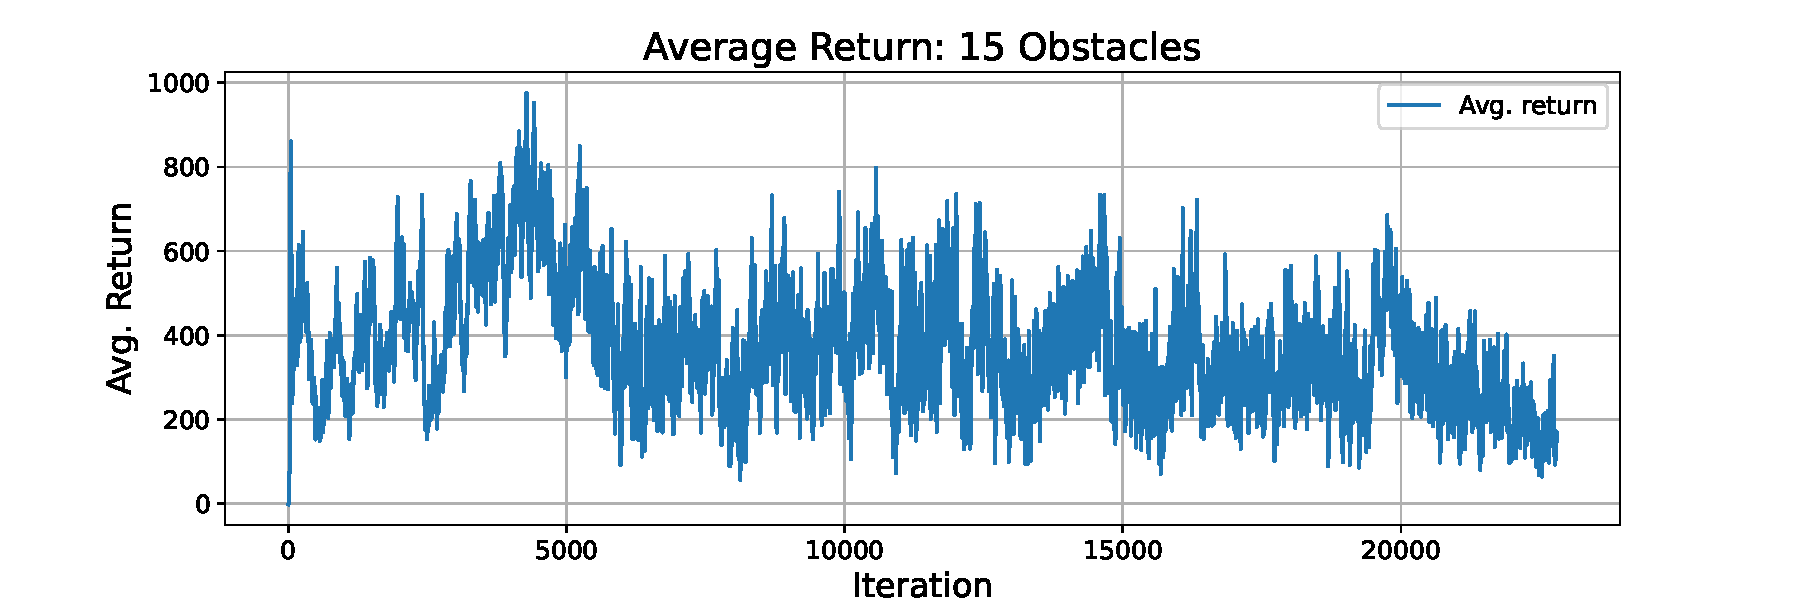
\includegraphics[width=0.98\textwidth]{figures/7_/3DCarModel_BodyObs_NavSetup_15_NewObs_EnvSpace12_best3190_v1_again_reward.pdf}
        \label{fig:15_obst_nav_rew}
    \end{subfigure} \\
    \begin{subfigure}[b]{\textwidth}
        \centering
        \captionsetup{justification=centering}
        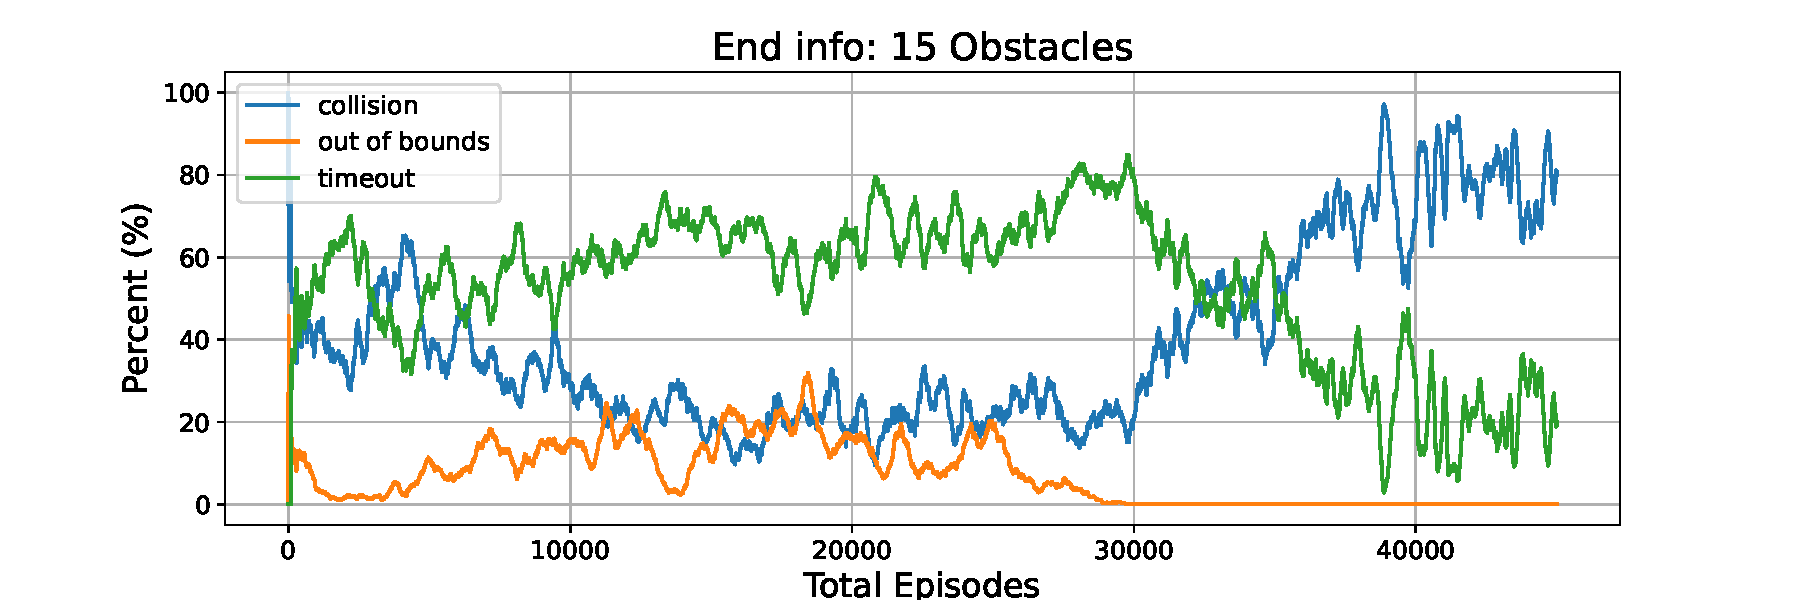
\includegraphics[width=0.98\textwidth]{figures/7_/3DCarModel_BodyObs_NavSetup_15_NewObs_EnvSpace12_best3190_v1_again_end_info.pdf}
        \label{fig:15_obst_nav_end}
    \end{subfigure} 
    \\
    \centering
    \begin{subfigure}[b]{\textwidth}
        \centering
        \captionsetup{justification=centering}
        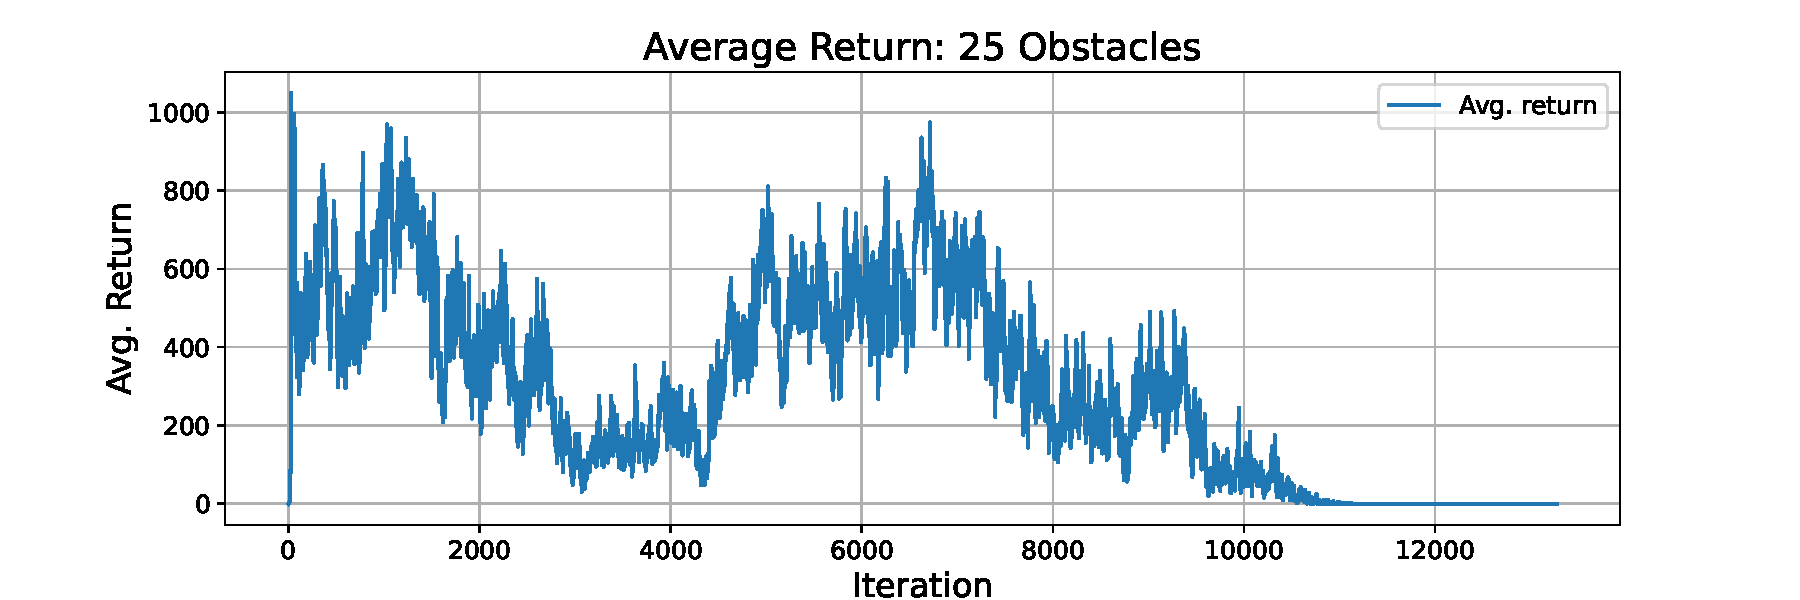
\includegraphics[width=0.98\textwidth]{figures/7_/3DCarModel_BodyObs_NavSetup_25_NewObs_EnvSpace15_last7600_v1_again_reward.pdf}
        \label{fig:25_obst_nav_rew}
    \end{subfigure} \\
    \begin{subfigure}[b]{\textwidth}
        \centering
        \captionsetup{justification=centering}
        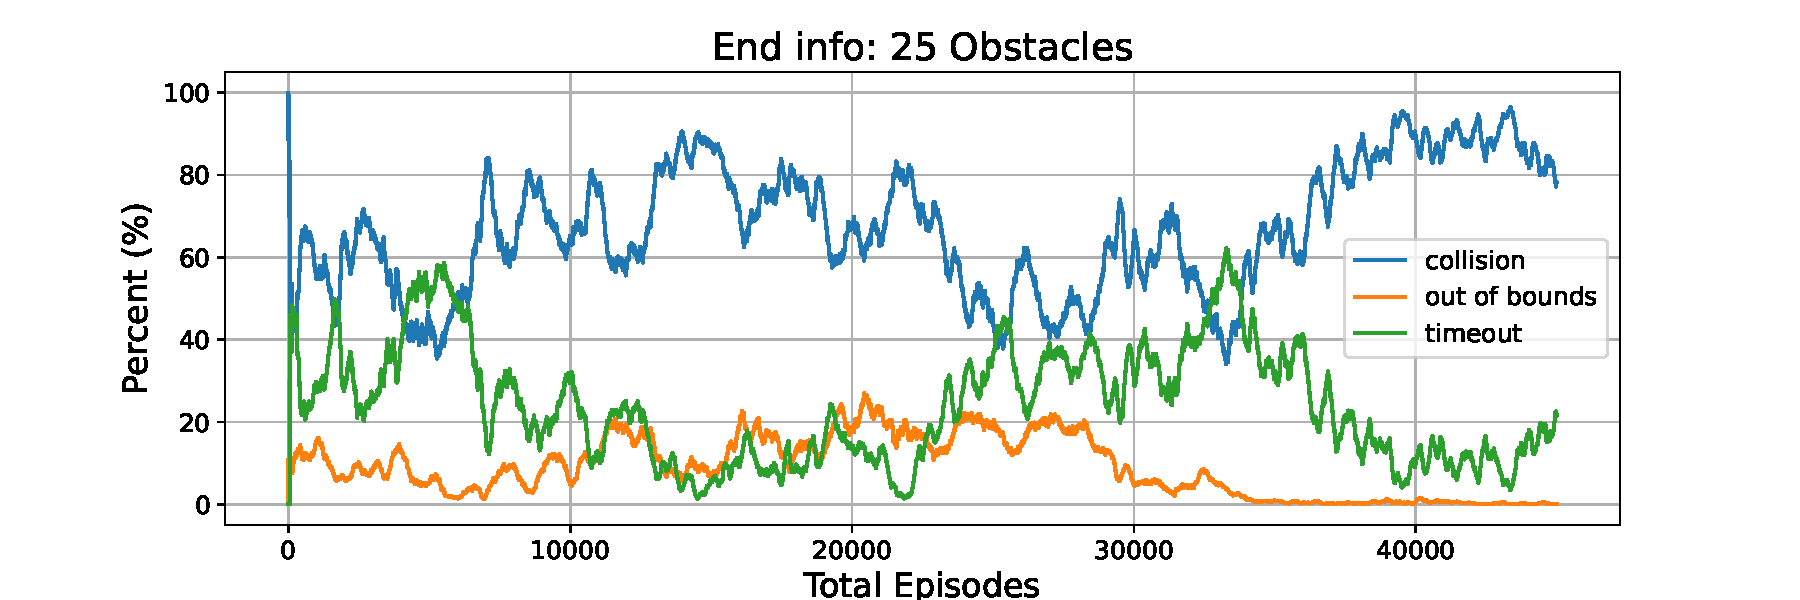
\includegraphics[width=0.98\textwidth]{figures/7_/3DCarModel_BodyObs_NavSetup_25_NewObs_EnvSpace15_last7600_v1_again_end_info.pdf}
        \label{fig:25_obst_nav_end}
    \end{subfigure} 
    \caption{Training the navigation policy with 15 and 25 obstacles in environments of size  $[24, 12]$ and $[30, 15]$, respectively. The best models were selected at 4410 and 6550 iterations.}
    \label{fig:7_train_nav_25_obst}
\end{figure}
\chapter{Environments}
\label{app:environments}

\end{document}
